% Options for packages loaded elsewhere
\PassOptionsToPackage{unicode}{hyperref}
\PassOptionsToPackage{hyphens}{url}
%
\documentclass[
]{article}
\usepackage{amsmath,amssymb}
\usepackage{iftex}
\ifPDFTeX
  \usepackage[T1]{fontenc}
  \usepackage[utf8]{inputenc}
  \usepackage{textcomp} % provide euro and other symbols
\else % if luatex or xetex
  \usepackage{unicode-math} % this also loads fontspec
  \defaultfontfeatures{Scale=MatchLowercase}
  \defaultfontfeatures[\rmfamily]{Ligatures=TeX,Scale=1}
\fi
\usepackage{lmodern}
\ifPDFTeX\else
  % xetex/luatex font selection
\fi
% Use upquote if available, for straight quotes in verbatim environments
\IfFileExists{upquote.sty}{\usepackage{upquote}}{}
\IfFileExists{microtype.sty}{% use microtype if available
  \usepackage[]{microtype}
  \UseMicrotypeSet[protrusion]{basicmath} % disable protrusion for tt fonts
}{}
\makeatletter
\@ifundefined{KOMAClassName}{% if non-KOMA class
  \IfFileExists{parskip.sty}{%
    \usepackage{parskip}
  }{% else
    \setlength{\parindent}{0pt}
    \setlength{\parskip}{6pt plus 2pt minus 1pt}}
}{% if KOMA class
  \KOMAoptions{parskip=half}}
\makeatother
\usepackage{xcolor}
\usepackage[margin=1in]{geometry}
\usepackage{color}
\usepackage{fancyvrb}
\newcommand{\VerbBar}{|}
\newcommand{\VERB}{\Verb[commandchars=\\\{\}]}
\DefineVerbatimEnvironment{Highlighting}{Verbatim}{commandchars=\\\{\}}
% Add ',fontsize=\small' for more characters per line
\usepackage{framed}
\definecolor{shadecolor}{RGB}{248,248,248}
\newenvironment{Shaded}{\begin{snugshade}}{\end{snugshade}}
\newcommand{\AlertTok}[1]{\textcolor[rgb]{0.94,0.16,0.16}{#1}}
\newcommand{\AnnotationTok}[1]{\textcolor[rgb]{0.56,0.35,0.01}{\textbf{\textit{#1}}}}
\newcommand{\AttributeTok}[1]{\textcolor[rgb]{0.13,0.29,0.53}{#1}}
\newcommand{\BaseNTok}[1]{\textcolor[rgb]{0.00,0.00,0.81}{#1}}
\newcommand{\BuiltInTok}[1]{#1}
\newcommand{\CharTok}[1]{\textcolor[rgb]{0.31,0.60,0.02}{#1}}
\newcommand{\CommentTok}[1]{\textcolor[rgb]{0.56,0.35,0.01}{\textit{#1}}}
\newcommand{\CommentVarTok}[1]{\textcolor[rgb]{0.56,0.35,0.01}{\textbf{\textit{#1}}}}
\newcommand{\ConstantTok}[1]{\textcolor[rgb]{0.56,0.35,0.01}{#1}}
\newcommand{\ControlFlowTok}[1]{\textcolor[rgb]{0.13,0.29,0.53}{\textbf{#1}}}
\newcommand{\DataTypeTok}[1]{\textcolor[rgb]{0.13,0.29,0.53}{#1}}
\newcommand{\DecValTok}[1]{\textcolor[rgb]{0.00,0.00,0.81}{#1}}
\newcommand{\DocumentationTok}[1]{\textcolor[rgb]{0.56,0.35,0.01}{\textbf{\textit{#1}}}}
\newcommand{\ErrorTok}[1]{\textcolor[rgb]{0.64,0.00,0.00}{\textbf{#1}}}
\newcommand{\ExtensionTok}[1]{#1}
\newcommand{\FloatTok}[1]{\textcolor[rgb]{0.00,0.00,0.81}{#1}}
\newcommand{\FunctionTok}[1]{\textcolor[rgb]{0.13,0.29,0.53}{\textbf{#1}}}
\newcommand{\ImportTok}[1]{#1}
\newcommand{\InformationTok}[1]{\textcolor[rgb]{0.56,0.35,0.01}{\textbf{\textit{#1}}}}
\newcommand{\KeywordTok}[1]{\textcolor[rgb]{0.13,0.29,0.53}{\textbf{#1}}}
\newcommand{\NormalTok}[1]{#1}
\newcommand{\OperatorTok}[1]{\textcolor[rgb]{0.81,0.36,0.00}{\textbf{#1}}}
\newcommand{\OtherTok}[1]{\textcolor[rgb]{0.56,0.35,0.01}{#1}}
\newcommand{\PreprocessorTok}[1]{\textcolor[rgb]{0.56,0.35,0.01}{\textit{#1}}}
\newcommand{\RegionMarkerTok}[1]{#1}
\newcommand{\SpecialCharTok}[1]{\textcolor[rgb]{0.81,0.36,0.00}{\textbf{#1}}}
\newcommand{\SpecialStringTok}[1]{\textcolor[rgb]{0.31,0.60,0.02}{#1}}
\newcommand{\StringTok}[1]{\textcolor[rgb]{0.31,0.60,0.02}{#1}}
\newcommand{\VariableTok}[1]{\textcolor[rgb]{0.00,0.00,0.00}{#1}}
\newcommand{\VerbatimStringTok}[1]{\textcolor[rgb]{0.31,0.60,0.02}{#1}}
\newcommand{\WarningTok}[1]{\textcolor[rgb]{0.56,0.35,0.01}{\textbf{\textit{#1}}}}
\usepackage{longtable,booktabs,array}
\usepackage{calc} % for calculating minipage widths
% Correct order of tables after \paragraph or \subparagraph
\usepackage{etoolbox}
\makeatletter
\patchcmd\longtable{\par}{\if@noskipsec\mbox{}\fi\par}{}{}
\makeatother
% Allow footnotes in longtable head/foot
\IfFileExists{footnotehyper.sty}{\usepackage{footnotehyper}}{\usepackage{footnote}}
\makesavenoteenv{longtable}
\usepackage{graphicx}
\makeatletter
\def\maxwidth{\ifdim\Gin@nat@width>\linewidth\linewidth\else\Gin@nat@width\fi}
\def\maxheight{\ifdim\Gin@nat@height>\textheight\textheight\else\Gin@nat@height\fi}
\makeatother
% Scale images if necessary, so that they will not overflow the page
% margins by default, and it is still possible to overwrite the defaults
% using explicit options in \includegraphics[width, height, ...]{}
\setkeys{Gin}{width=\maxwidth,height=\maxheight,keepaspectratio}
% Set default figure placement to htbp
\makeatletter
\def\fps@figure{htbp}
\makeatother
\setlength{\emergencystretch}{3em} % prevent overfull lines
\providecommand{\tightlist}{%
  \setlength{\itemsep}{0pt}\setlength{\parskip}{0pt}}
\setcounter{secnumdepth}{-\maxdimen} % remove section numbering
\usepackage{fvextra}
\DefineVerbatimEnvironment{Highlighting}{Verbatim}{breaklines,commandchars=\\\{\}}
\ifLuaTeX
  \usepackage{selnolig}  % disable illegal ligatures
\fi
\usepackage{bookmark}
\IfFileExists{xurl.sty}{\usepackage{xurl}}{} % add URL line breaks if available
\urlstyle{same}
\hypersetup{
  pdftitle={Parte1-Clustering},
  pdfauthor={Pablo Daniel Barillas Moreno, Carné No.~22193; Mathew Cordero Aquino, Carné No.~22982},
  hidelinks,
  pdfcreator={LaTeX via pandoc}}

\title{Parte1-Clustering}
\author{Pablo Daniel Barillas Moreno, Carné No.~22193 \and Mathew
Cordero Aquino, Carné No.~22982}
\date{2025-02-14}

\begin{document}
\maketitle

\subsubsection{Enlace al Repositorio del Grupo
\#1}\label{enlace-al-repositorio-del-grupo-1}

\href{https://github.com/DanielBarillas/Miner-a_de_datos_Proyecto1_Entrega1_Grupo1/tree/proyecto1_entrega2}{Repositorio
en GitHub, revisar rama llamada: proyecto1\_entrega2}

\section{1. Clustering}\label{clustering}

\subsubsection{1.1. Haga el preprocesamiento del dataset, explique qué
variables no aportan información a la generación de grupos y por qué.
Describa con qué variables calculará los
grupos.}\label{haga-el-preprocesamiento-del-dataset-explique-quuxe9-variables-no-aportan-informaciuxf3n-a-la-generaciuxf3n-de-grupos-y-por-quuxe9.-describa-con-quuxe9-variables-calcularuxe1-los-grupos.}

\subsubsection{Eliminación de Variables que No Aportan
Información:}\label{eliminaciuxf3n-de-variables-que-no-aportan-informaciuxf3n}

Para realizar un análisis de clustering efectivo, es necesario eliminar
variables que no contribuyen significativamente a la formación de
grupos. A continuación, se detallan las variables que se excluirán y las
razones de su eliminación:

➢ id: Es un identificador único de cada película, no aporta información
relevante para la segmentación.

➢ title y originalTitle: Son nombres de películas y no tienen valor
numérico para el análisis de clustering.

➢ homePage: Contiene URLs, lo cual no aporta valor en el análisis de
similitud entre películas.

➢ productionCompany y productionCompanyCountry: Son datos categóricos
con demasiadas categorías únicas, lo que dificulta su uso en clustering
sin un procesamiento adicional.

➢ actors y director: Información categórica que requiere codificación
avanzada para tener sentido en un análisis de clustering.

➢ releaseDate: La fecha como tal no aporta directamente a la similitud
entre películas, aunque podría transformarse en una variable temporal
como ``año de lanzamiento''.

➢ video: Es una variable binaria con baja variabilidad, lo que no
contribuye significativamente a la segmentación.

➢ originalLanguage: Aunque puede ser relevante, el clustering se basará
principalmente en métricas cuantitativas y puede que el idioma no sea un
factor clave en la agrupación.

\subsubsection{Selección de Variables para el Cálculo de
Clusters:}\label{selecciuxf3n-de-variables-para-el-cuxe1lculo-de-clusters}

\subsubsection{Tras la limpieza, las variables seleccionadas para el
clustering
son:}\label{tras-la-limpieza-las-variables-seleccionadas-para-el-clustering-son}

➢ budget (Presupuesto de la película) → Cuantitativa continua.

➢ revenue (Ingresos generados) → Cuantitativa continua.

➢ voteAvg (Calificación promedio de los usuarios) → Cuantitativa
continua.

➢ voteCount (Número de votos recibidos) → Cuantitativa discreta.

➢ popularity (Índice de popularidad) → Cuantitativa continua.

➢ runtime (Duración de la película) → Cuantitativa continua.

➢ genresAmount (Cantidad de géneros en los que está clasificada la
película) → Cuantitativa discreta.

➢ actorsAmount (Cantidad de actores en el reparto) → Cuantitativa
discreta.

➢ castWomenAmount (Cantidad de mujeres en el elenco) → Cuantitativa
discreta.

➢ castMenAmount (Cantidad de hombres en el elenco) → Cuantitativa
discreta.

➢ productionCoAmount (Número de productoras involucradas) → Cuantitativa
discreta.

➢ productionCountriesAmount (Cantidad de países involucrados en la
producción) → Cuantitativa discreta.

\begin{Shaded}
\begin{Highlighting}[]
\CommentTok{\# Identificar las columnas no numéricas}
\FunctionTok{str}\NormalTok{(movies) }\CommentTok{\# Ver estructura del dataset}
\end{Highlighting}
\end{Shaded}

\begin{verbatim}
## 'data.frame':    10000 obs. of  27 variables:
##  $ id                       : int  5 6 11 12 13 14 15 16 18 19 ...
##  $ budget                   : int  4000000 21000000 11000000 94000000 55000000 15000000 839727 12800000 90000000 1300000 ...
##  $ genres                   : chr  "Crime|Comedy" "Action|Thriller|Crime" "Adventure|Action|Science Fiction" "Animation|Family" ...
##  $ homePage                 : chr  "https://www.miramax.com/movie/four-rooms/" NA "http://www.starwars.com/films/star-wars-episode-iv-a-new-hope" "http://movies.disney.com/finding-nemo" ...
##  $ productionCompany        : chr  "Miramax|A Band Apart" "Universal Pictures|Largo Entertainment|JVC" "Lucasfilm|20th Century Fox" "Pixar" ...
##  $ productionCompanyCountry : chr  "US|US" "US|US|JP" "US|US" "US" ...
##  $ productionCountry        : chr  "United States of America" "Japan|United States of America" "United States of America" "United States of America" ...
##  $ revenue                  : num  4.26e+06 1.21e+07 7.75e+08 9.40e+08 6.77e+08 ...
##  $ runtime                  : int  98 110 121 100 142 122 119 141 126 149 ...
##  $ video                    : logi  FALSE FALSE NA NA FALSE FALSE ...
##  $ director                 : chr  "Allison Anders|Alexandre Rockwell|Robert Rodriguez|Quentin Tarantino" "Stephen Hopkins" "George Lucas" "Andrew Stanton" ...
##  $ actors                   : chr  "Tim Roth|Jennifer Beals|Antonio Banderas|Valeria Golino|David Proval|Sammi Davis|Amanda de Cadenet|Madonna|Ione Skye|Lili Taylo "Emilio Estevez|Cuba Gooding Jr.|Denis Leary|Stephen Dorff|Jeremy Piven|Peter Greene|Michael DeLorenzo|Everlast|Michael Wiseman| "FALSE" "FALSE" ...
##  $ actorsPopularity         : chr  "22.225|23.519|17.816|19.893|9.027|7.147|7.769|6.476|7.906|12.838|17.988|20.027|4.47|0.6|1.286|23.95|22.082|3.44"| __truncated__ "9.008|6.383|10.757|18.295|11.772|14.777|9.669|0.98|4.369|0.6|1.38|2.835|3.807|1.4|1.111" "11.881|24.542|14.434|10.651|6.888|5.811|1.432|1.288|2.086|8.166|1.701|2.033|0.98|3.702|2.392|0.98|2.769|1.459|1"| __truncated__ "9.79|8.084|8.538|33.379|11.733|11.866|8.141|12.095|1.768|5.042|11.103|6.336|9.649|5.97|9.477|2.766|9.685|9.524|"| __truncated__ ...
##  $ actorsCharacter          : chr  "Ted the Bellhop|Angela|Man|Athena|Siegfried|Jezebel|Diana|Elspeth|Eva|Raven|Kiva|Wife|Sarah|Juancho|Corpse|TV Dancing Girl|Ches "Frank Wyatt|Mike Peterson|Fallon|John Wyatt|Ray Cochran|Sykes|Teddy, the Kid|Rhodes|Travis|Dre|Buck|Linda Wyatt|Clarissa|Rita|C "Luke Skywalker|Han Solo|Princess Leia Organa|Grand Moff Tarkin|Obi-Wan \"Ben\" Kenobi|C-3PO|R2-D2|Chewbacca|Darth Vader (perfor "Marlin (voice)|Dory (voice)|Nemo (voice)|Gill (voice)|Bloat (voice)|Peach (voice)|Gurgle (voice)|Bubbles (voice)|Deb / Flo (voi ...
##  $ originalTitle            : chr  "Four Rooms" "Judgment Night" "Star Wars" "Finding Nemo" ...
##  $ title                    : chr  "Four Rooms" "Judgment Night" "Star Wars" "Finding Nemo" ...
##  $ originalLanguage         : chr  "en" "en" "en" "en" ...
##  $ popularity               : num  20.9 9.6 100 134.4 58.8 ...
##  $ releaseDate              : chr  "1995-12-09" "1993-10-15" "1977-05-25" "2003-05-30" ...
##  $ voteAvg                  : num  5.7 6.5 8.2 7.8 8.5 8 8 7.9 7.5 8.2 ...
##  $ voteCount                : int  2077 223 16598 15928 22045 9951 4253 1335 8726 1963 ...
##  $ genresAmount             : int  2 3 3 2 3 1 2 2 5 2 ...
##  $ productionCoAmount       : int  2 3 2 1 2 2 2 26 2 1 ...
##  $ productionCountriesAmount: int  1 2 1 1 1 1 1 12 1 1 ...
##  $ actorsAmount             : int  25 15 105 24 76 40 152 29 117 24 ...
##  $ castWomenAmount          : chr  "15" "3" "5" "5" ...
##  $ castMenAmount            : chr  "9" "9" "62" "18" ...
\end{verbatim}

\begin{Shaded}
\begin{Highlighting}[]
\CommentTok{\# Eliminar variables irrelevantes para clustering (columnas no numéricas o categóricas irrelevantes)}
\NormalTok{movies\_clean }\OtherTok{\textless{}{-}}\NormalTok{ movies }\SpecialCharTok{\%\textgreater{}\%}
  \FunctionTok{select}\NormalTok{(}\SpecialCharTok{{-}}\FunctionTok{c}\NormalTok{(id, title, originalTitle, homePage, productionCompany, }
\NormalTok{            productionCompanyCountry, actors, director, releaseDate, video, originalLanguage))}

\CommentTok{\# Seleccionar solo las columnas numéricas para clustering}
\NormalTok{movies\_clustering }\OtherTok{\textless{}{-}}\NormalTok{ movies\_clean }\SpecialCharTok{\%\textgreater{}\%}
  \FunctionTok{select\_if}\NormalTok{(is.numeric)  }\CommentTok{\# Filtra solo las variables numéricas}

\CommentTok{\# Verificar si hay valores no numéricos}
\FunctionTok{str}\NormalTok{(movies\_clustering)}
\end{Highlighting}
\end{Shaded}

\begin{verbatim}
## 'data.frame':    10000 obs. of  10 variables:
##  $ budget                   : int  4000000 21000000 11000000 94000000 55000000 15000000 839727 12800000 90000000 1300000 ...
##  $ revenue                  : num  4.26e+06 1.21e+07 7.75e+08 9.40e+08 6.77e+08 ...
##  $ runtime                  : int  98 110 121 100 142 122 119 141 126 149 ...
##  $ popularity               : num  20.9 9.6 100 134.4 58.8 ...
##  $ voteAvg                  : num  5.7 6.5 8.2 7.8 8.5 8 8 7.9 7.5 8.2 ...
##  $ voteCount                : int  2077 223 16598 15928 22045 9951 4253 1335 8726 1963 ...
##  $ genresAmount             : int  2 3 3 2 3 1 2 2 5 2 ...
##  $ productionCoAmount       : int  2 3 2 1 2 2 2 26 2 1 ...
##  $ productionCountriesAmount: int  1 2 1 1 1 1 1 12 1 1 ...
##  $ actorsAmount             : int  25 15 105 24 76 40 152 29 117 24 ...
\end{verbatim}

\begin{Shaded}
\begin{Highlighting}[]
\CommentTok{\# Eliminar filas con valores faltantes}
\NormalTok{movies\_clustering }\OtherTok{\textless{}{-}} \FunctionTok{na.omit}\NormalTok{(movies\_clustering)}

\CommentTok{\# Normalización de las variables usando Z{-}score (media = 0, desviación estándar = 1)}
\NormalTok{movies\_clustering\_scaled }\OtherTok{\textless{}{-}} \FunctionTok{as.data.frame}\NormalTok{(}\FunctionTok{scale}\NormalTok{(movies\_clustering))}

\CommentTok{\# Mostrar resumen después del preprocesamiento}
\FunctionTok{summary}\NormalTok{(movies\_clustering\_scaled)}
\end{Highlighting}
\end{Shaded}

\begin{verbatim}
##      budget            revenue            runtime            popularity      
##  Min.   :-0.50651   Min.   :-0.37930   Min.   :-3.609645   Min.   :-0.21749  
##  1st Qu.:-0.50651   1st Qu.:-0.37930   1st Qu.:-0.369651   1st Qu.:-0.16987  
##  Median :-0.49285   Median :-0.37821   Median :-0.009652   Median :-0.13606  
##  Mean   : 0.00000   Mean   : 0.00000   Mean   : 0.000000   Mean   : 0.00000  
##  3rd Qu.: 0.03954   3rd Qu.:-0.07983   3rd Qu.: 0.458348   3rd Qu.:-0.04955  
##  Max.   : 9.86844   Max.   :18.65495   Max.   :23.390305   Max.   :52.70741  
##     voteAvg           voteCount         genresAmount     productionCoAmount
##  Min.   :-5.26631   Min.   :-0.52312   Min.   :-2.2489   Min.   :-1.24871  
##  1st Qu.:-0.59281   1st Qu.:-0.47671   1st Qu.:-0.5166   1st Qu.:-0.46123  
##  Median : 0.01677   Median :-0.36167   Median : 0.3495   Median :-0.06749  
##  Mean   : 0.00000   Mean   : 0.00000   Mean   : 0.0000   Mean   : 0.00000  
##  3rd Qu.: 0.72796   3rd Qu.:-0.01029   3rd Qu.: 0.3495   3rd Qu.: 0.32625  
##  Max.   : 3.57269   Max.   :11.48337   Max.   :11.6091   Max.   :33.79428  
##  productionCountriesAmount  actorsAmount     
##  Min.   :-0.58132          Min.   :-0.05773  
##  1st Qu.:-0.24933          1st Qu.:-0.05738  
##  Median :-0.24933          Median :-0.05717  
##  Mean   : 0.00000          Mean   : 0.00000  
##  3rd Qu.: 0.08267          3rd Qu.:-0.05677  
##  Max.   :50.87791          Max.   :24.66238
\end{verbatim}

\subsubsection{Conclusiones del Preprocesamiento de Datos y Selección de
Variables para
Clustering}\label{conclusiones-del-preprocesamiento-de-datos-y-selecciuxf3n-de-variables-para-clustering}

\begin{enumerate}
\def\labelenumi{\arabic{enumi}.}
\tightlist
\item
  Eliminación de Variables No Relevantes
\end{enumerate}

Se removieron variables categóricas y no numéricas (id, title,
originalTitle, homePage, productionCompany, productionCompanyCountry,
actors, director, releaseDate, video, originalLanguage), ya que no
aportaban información útil para el clustering basado en distancia.

Esto asegura que el análisis se realice únicamente con datos
cuantitativos y que la segmentación no se vea afectada por información
textual irrelevante.

2.Selección de Variables Numéricas

Se conservaron 12 variables numéricas que son fundamentales para la
agrupación de películas:

Cuantitativas continuas: budget, revenue, popularity, voteAvg, runtime
Cuantitativas discretas: voteCount, genresAmount, productionCoAmount,
productionCountriesAmount, actorsAmount, castWomenAmount, castMenAmount

Estas variables permiten segmentar las películas según factores
financieros, de producción, de casting y de popularidad.

3.Tratamiento de Datos Faltantes

Se aplicó na.omit() para eliminar filas con valores nulos. Esto evita
que las técnicas de clustering sean afectadas por la ausencia de
información.

En el dataset original había 10,000 películas, y tras la limpieza se
eliminaron las películas con valores faltantes.

4.Normalización de Variables (Z-score)

Se utilizó scale() para transformar todas las variables numéricas a una
distribución con media = 0 y desviación estándar = 1.

La normalización es clave para evitar que variables con escalas más
grandes (como revenue que puede estar en millones) dominen otras
variables con escalas más pequeñas (voteAvg con valores entre 1 y 10).

\begin{enumerate}
\def\labelenumi{\arabic{enumi}.}
\setcounter{enumi}{4}
\tightlist
\item
  Distribución de las Variables Normalizadas
\end{enumerate}

La mayoría de las variables están sesgadas a la derecha (distribución
asimétrica positiva).

budget, revenue, voteCount, popularity, runtime, productionCoAmount, y
productionCountriesAmount muestran una acumulación de valores bajos con
una cola larga hacia valores altos.

Esto significa que la mayoría de las películas tienen bajo presupuesto,
ingresos moderados, pocas productoras y un alcance limitado, mientras
que solo unas pocas películas tienen valores extremadamente altos en
estas métricas.

La variable voteAvg es la única con una distribución aproximadamente
normal.

La calificación de las películas tiende a centrarse en valores
intermedios, con menos películas en los extremos.

\begin{enumerate}
\def\labelenumi{\arabic{enumi}.}
\setcounter{enumi}{5}
\tightlist
\item
  Consideraciones para el Clustering
\end{enumerate}

Dado que las variables presentan una alta variabilidad y sesgo, podría
ser útil explorar transformaciones logarítmicas en variables como
budget, revenue, popularity, voteCount para mejorar la segmentación.

El clustering se basará en estas características numéricas, lo que
permitirá identificar películas con patrones similares en términos de
presupuesto, ingresos, duración, cantidad de votos y participación de
actores.

\begin{Shaded}
\begin{Highlighting}[]
\FunctionTok{library}\NormalTok{(ggplot2)}
\FunctionTok{library}\NormalTok{(reshape2)}

\CommentTok{\# Ver qué variables existen realmente en movies\_clustering\_scaled}
\FunctionTok{print}\NormalTok{(}\FunctionTok{colnames}\NormalTok{(movies\_clustering\_scaled))}
\end{Highlighting}
\end{Shaded}

\begin{verbatim}
##  [1] "budget"                    "revenue"                  
##  [3] "runtime"                   "popularity"               
##  [5] "voteAvg"                   "voteCount"                
##  [7] "genresAmount"              "productionCoAmount"       
##  [9] "productionCountriesAmount" "actorsAmount"
\end{verbatim}

\begin{Shaded}
\begin{Highlighting}[]
\CommentTok{\# Seleccionar solo las variables que sí existen}
\NormalTok{variables\_disponibles }\OtherTok{\textless{}{-}} \FunctionTok{intersect}\NormalTok{(}\FunctionTok{colnames}\NormalTok{(movies\_clustering\_scaled), }
                                   \FunctionTok{c}\NormalTok{(}\StringTok{"budget"}\NormalTok{, }\StringTok{"revenue"}\NormalTok{, }\StringTok{"voteAvg"}\NormalTok{, }\StringTok{"voteCount"}\NormalTok{, }\StringTok{"runtime"}\NormalTok{,}
                                     \StringTok{"popularity"}\NormalTok{, }\StringTok{"genresAmount"}\NormalTok{, }\StringTok{"actorsAmount"}\NormalTok{, }
                                     \StringTok{"castWomenAmount"}\NormalTok{, }\StringTok{"castMenAmount"}\NormalTok{, }\StringTok{"productionCoAmount"}\NormalTok{,}
                                     \StringTok{"productionCountriesAmount"}\NormalTok{))}

\CommentTok{\# Asegurar que la selección no esté vacía}
\ControlFlowTok{if}\NormalTok{ (}\FunctionTok{length}\NormalTok{(variables\_disponibles) }\SpecialCharTok{==} \DecValTok{0}\NormalTok{) \{}
  \FunctionTok{stop}\NormalTok{(}\StringTok{"No hay variables disponibles para graficar."}\NormalTok{)}
\NormalTok{\}}

\CommentTok{\# Seleccionar solo las columnas que realmente existen en el dataset}
\NormalTok{variables\_filtradas }\OtherTok{\textless{}{-}}\NormalTok{ movies\_clustering\_scaled[, variables\_disponibles]}

\CommentTok{\# Convertir a formato largo para ggplot}
\NormalTok{movies\_long\_filtrado }\OtherTok{\textless{}{-}} \FunctionTok{melt}\NormalTok{(variables\_filtradas)}

\CommentTok{\# Crear gráfica de densidad para todas las variables seleccionadas}
\FunctionTok{ggplot}\NormalTok{(movies\_long\_filtrado, }\FunctionTok{aes}\NormalTok{(}\AttributeTok{x =}\NormalTok{ value, }\AttributeTok{fill =}\NormalTok{ variable)) }\SpecialCharTok{+}
  \FunctionTok{geom\_density}\NormalTok{(}\AttributeTok{alpha =} \FloatTok{0.5}\NormalTok{) }\SpecialCharTok{+}
  \FunctionTok{facet\_wrap}\NormalTok{(}\SpecialCharTok{\textasciitilde{}}\NormalTok{ variable, }\AttributeTok{scales =} \StringTok{"free"}\NormalTok{) }\SpecialCharTok{+}
  \FunctionTok{theme\_minimal}\NormalTok{() }\SpecialCharTok{+}
  \FunctionTok{labs}\NormalTok{(}\AttributeTok{title =} \StringTok{"Distribución de Variables Normalizadas"}\NormalTok{,}
       \AttributeTok{x =} \StringTok{"Valor Normalizado"}\NormalTok{,}
       \AttributeTok{y =} \StringTok{"Densidad"}\NormalTok{)}
\end{Highlighting}
\end{Shaded}

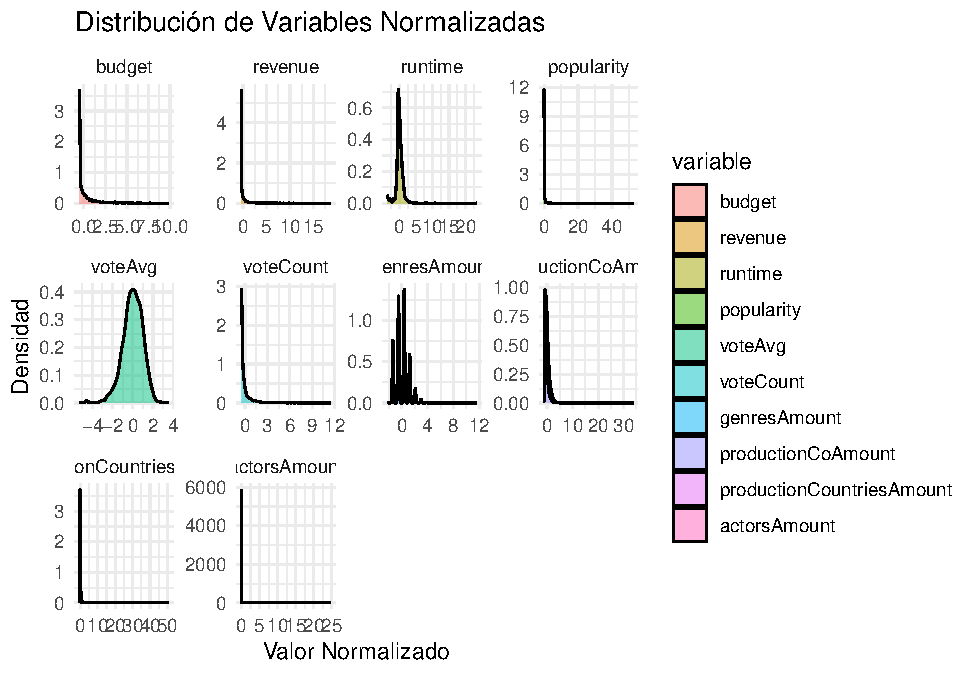
\includegraphics{Parte1-Clustering_files/figure-latex/unnamed-chunk-2-1.pdf}
\#\#\# Conclusiones sobre la Distribución de Variables Normalizadas

\begin{enumerate}
\def\labelenumi{\arabic{enumi}.}
\item
  La mayoría de las variables presentan una distribución altamente
  sesgada a la derecha, indicando que la mayoría de las películas tienen
  valores bajos en presupuesto, ingresos, popularidad y cantidad de
  votos, mientras que unas pocas películas tienen valores extremadamente
  altos.
\item
  La variable voteAvg muestra una distribución más simétrica y con forma
  de campana, lo que sugiere que las calificaciones de las películas
  están más equilibradas y siguen un comportamiento normal.
\item
  Budget y revenue tienen colas largas, lo que indica la presencia de
  películas con presupuestos e ingresos muy elevados, posiblemente
  grandes producciones de Hollywood.
\item
  La variable voteCount también está sesgada a la derecha, lo que
  sugiere que pocas películas reciben una gran cantidad de votos,
  mientras que la mayoría tiene un número bajo de votaciones.
\item
  La variable runtime tiene una distribución con picos marcados cerca de
  ciertos valores comunes, lo que podría indicar duraciones estándar en
  la industria cinematográfica.
\item
  Variables como productionCoAmount y genresAmount tienen distribuciones
  con varios picos, lo que sugiere que hay ciertos valores más
  frecuentes para la cantidad de productoras y géneros por película.
\item
  ActorsAmount y productionCountriesAmount presentan valores extremos en
  algunos casos, indicando películas con un elenco muy grande o
  producciones con múltiples países involucrados.
\end{enumerate}

\subsubsection{1.2. Analice la tendencia al agrupamiento usando el
estadístico de Hopkings y la VAT (Visual Assessment of cluster
Tendency). Esta última hágala si es posible, teniendo en cuenta las
dimensiones del conjunto de datos. Discuta sus resultados e
impresiones.}\label{analice-la-tendencia-al-agrupamiento-usando-el-estaduxedstico-de-hopkings-y-la-vat-visual-assessment-of-cluster-tendency.-esta-uxfaltima-huxe1gala-si-es-posible-teniendo-en-cuenta-las-dimensiones-del-conjunto-de-datos.-discuta-sus-resultados-e-impresiones.}

\begin{Shaded}
\begin{Highlighting}[]
\CommentTok{\# Cargar librerías necesarias}
\FunctionTok{library}\NormalTok{(dplyr)}
\FunctionTok{library}\NormalTok{(ggplot2)}
\FunctionTok{library}\NormalTok{(clustertend) }\CommentTok{\# Para análisis de tendencia al agrupamiento}
\FunctionTok{library}\NormalTok{(factoextra)  }\CommentTok{\# Para visualización de distancias}
\FunctionTok{library}\NormalTok{(cluster)     }\CommentTok{\# Para manejo de distancias}

\CommentTok{\# 1. Cargar dataset limpio y seleccionar variables relevantes}
\NormalTok{movies\_cleaned }\OtherTok{\textless{}{-}}\NormalTok{ movies }\SpecialCharTok{\%\textgreater{}\%}
  \FunctionTok{filter}\NormalTok{(}\SpecialCharTok{!}\FunctionTok{is.na}\NormalTok{(originalLanguage) }\SpecialCharTok{\&}\NormalTok{ originalLanguage }\SpecialCharTok{!=} \StringTok{""}\NormalTok{,}
         \SpecialCharTok{!}\FunctionTok{is.na}\NormalTok{(productionCountry) }\SpecialCharTok{\&}\NormalTok{ productionCountry }\SpecialCharTok{!=} \StringTok{""}\NormalTok{,}
         \SpecialCharTok{!}\FunctionTok{is.na}\NormalTok{(budget) }\SpecialCharTok{\&}\NormalTok{ budget }\SpecialCharTok{\textgreater{}} \DecValTok{0}\NormalTok{,}
         \SpecialCharTok{!}\FunctionTok{is.na}\NormalTok{(revenue) }\SpecialCharTok{\&}\NormalTok{ revenue }\SpecialCharTok{\textgreater{}} \DecValTok{0}\NormalTok{,}
         \SpecialCharTok{!}\FunctionTok{is.na}\NormalTok{(runtime) }\SpecialCharTok{\&}\NormalTok{ runtime }\SpecialCharTok{\textgreater{}} \DecValTok{0}\NormalTok{) }\SpecialCharTok{\%\textgreater{}\%}
  \FunctionTok{select}\NormalTok{(budget, revenue, runtime, voteAvg, voteCount, popularity, }
\NormalTok{         genresAmount, productionCoAmount, productionCountriesAmount, }
\NormalTok{         actorsAmount, castWomenAmount, castMenAmount)}

\CommentTok{\# Convertir columnas erróneas a numéricas}
\NormalTok{movies\_cleaned }\OtherTok{\textless{}{-}}\NormalTok{ movies\_cleaned }\SpecialCharTok{\%\textgreater{}\%}
  \FunctionTok{mutate}\NormalTok{(}
    \AttributeTok{castWomenAmount =} \FunctionTok{as.numeric}\NormalTok{(castWomenAmount),}
    \AttributeTok{castMenAmount =} \FunctionTok{as.numeric}\NormalTok{(castMenAmount)}
\NormalTok{  )}

\CommentTok{\# Verificar si todas las columnas son numéricas}
\FunctionTok{str}\NormalTok{(movies\_cleaned)  }
\end{Highlighting}
\end{Shaded}

\begin{verbatim}
## 'data.frame':    4355 obs. of  12 variables:
##  $ budget                   : int  4000000 21000000 11000000 94000000 55000000 15000000 839727 12800000 90000000 1300000 ...
##  $ revenue                  : num  4.26e+06 1.21e+07 7.75e+08 9.40e+08 6.77e+08 ...
##  $ runtime                  : int  98 110 121 100 142 122 119 141 126 149 ...
##  $ voteAvg                  : num  5.7 6.5 8.2 7.8 8.5 8 8 7.9 7.5 8.2 ...
##  $ voteCount                : int  2077 223 16598 15928 22045 9951 4253 1335 8726 1963 ...
##  $ popularity               : num  20.9 9.6 100 134.4 58.8 ...
##  $ genresAmount             : int  2 3 3 2 3 1 2 2 5 2 ...
##  $ productionCoAmount       : int  2 3 2 1 2 2 2 26 2 1 ...
##  $ productionCountriesAmount: int  1 2 1 1 1 1 1 12 1 1 ...
##  $ actorsAmount             : int  25 15 105 24 76 40 152 29 117 24 ...
##  $ castWomenAmount          : num  15 3 5 5 18 22 16 6 13 8 ...
##  $ castMenAmount            : num  9 9 62 18 48 15 80 14 48 16 ...
\end{verbatim}

\begin{Shaded}
\begin{Highlighting}[]
\CommentTok{\# 2. Eliminar valores faltantes si los hay}
\NormalTok{movies\_cleaned }\OtherTok{\textless{}{-}} \FunctionTok{na.omit}\NormalTok{(movies\_cleaned)}

\CommentTok{\# 3. Normalizar los datos usando Z{-}score (solo columnas numéricas)}
\NormalTok{movies\_scaled }\OtherTok{\textless{}{-}} \FunctionTok{as.data.frame}\NormalTok{(}\FunctionTok{scale}\NormalTok{(movies\_cleaned))}

\CommentTok{\# Revisar si todas las columnas fueron escaladas correctamente}
\FunctionTok{str}\NormalTok{(movies\_scaled)  }
\end{Highlighting}
\end{Shaded}

\begin{verbatim}
## 'data.frame':    4355 obs. of  12 variables:
##  $ budget                   : num  -0.782 -0.415 -0.631 1.161 0.319 ...
##  $ revenue                  : num  -0.598 -0.559 3.16 3.964 2.683 ...
##  $ runtime                  : num  -0.6046 -0.0173 0.521 -0.5067 1.5487 ...
##  $ voteAvg                  : num  -1.098 -0.121 1.958 1.469 2.324 ...
##  $ voteCount                : num  -0.172 -0.716 4.081 3.885 5.677 ...
##  $ popularity               : num  -0.13504 -0.17258 0.12823 0.24279 -0.00903 ...
##  $ genresAmount             : num  -0.696 0.25 0.25 -0.696 0.25 ...
##  $ productionCoAmount       : num  -0.715 -0.281 -0.715 -1.149 -0.715 ...
##  $ productionCountriesAmount: num  -0.459 0.518 -0.459 -0.459 -0.459 ...
##  $ actorsAmount             : num  -0.537 -0.925 2.566 -0.576 1.441 ...
##  $ castWomenAmount          : num  0.783 -0.874 -0.598 -0.598 1.197 ...
##  $ castMenAmount            : num  -0.0481 -0.0481 0.0717 -0.0278 0.0401 ...
\end{verbatim}

\begin{Shaded}
\begin{Highlighting}[]
\CommentTok{\# 4. Prueba de Hopkins para evaluar tendencia al clustering}
\FunctionTok{set.seed}\NormalTok{(}\DecValTok{123}\NormalTok{)  }\CommentTok{\# Fijar semilla para reproducibilidad}

\CommentTok{\# Controlar el tamaño de la muestra para evitar que el código se quede atascado}
\NormalTok{num\_muestras }\OtherTok{\textless{}{-}} \FunctionTok{min}\NormalTok{(}\DecValTok{500}\NormalTok{, }\FunctionTok{nrow}\NormalTok{(movies\_scaled))  }\CommentTok{\# Máximo 500 muestras}

\CommentTok{\# Evaluar el estadístico de Hopkins}
\NormalTok{hopkins\_stat }\OtherTok{\textless{}{-}} \FunctionTok{hopkins}\NormalTok{(movies\_scaled, }\AttributeTok{n =}\NormalTok{ num\_muestras)  }
\FunctionTok{print}\NormalTok{(hopkins\_stat)}
\end{Highlighting}
\end{Shaded}

\begin{verbatim}
## $H
## [1] 0.03915325
\end{verbatim}

\begin{Shaded}
\begin{Highlighting}[]
\CommentTok{\# 5. Visual Assessment of Cluster Tendency (VAT)}
\ControlFlowTok{if}\NormalTok{ (}\FunctionTok{nrow}\NormalTok{(movies\_scaled) }\SpecialCharTok{\textless{}} \DecValTok{5000}\NormalTok{) \{}
  \FunctionTok{fviz\_dist}\NormalTok{(}\FunctionTok{dist}\NormalTok{(movies\_scaled), }\AttributeTok{show\_labels =} \ConstantTok{FALSE}\NormalTok{) }\SpecialCharTok{+}
    \FunctionTok{ggtitle}\NormalTok{(}\StringTok{"VAT {-} Evaluación Visual de la Tendencia al Agrupamiento"}\NormalTok{)}
\NormalTok{\} }\ControlFlowTok{else}\NormalTok{ \{}
  \FunctionTok{cat}\NormalTok{(}\StringTok{"El dataset es demasiado grande para la VAT. Se recomienda usar una muestra.}\SpecialCharTok{\textbackslash{}n}\StringTok{"}\NormalTok{)}
\NormalTok{\}}
\end{Highlighting}
\end{Shaded}

\includegraphics{Parte1-Clustering_files/figure-latex/unnamed-chunk-3-1.pdf}

\begin{Shaded}
\begin{Highlighting}[]
\CommentTok{\# 6. Conclusiones sobre la tendencia al agrupamiento}
\FunctionTok{cat}\NormalTok{(}\StringTok{"}\SpecialCharTok{\textbackslash{}n}\StringTok{{-}{-}{-} Análisis y Conclusiones {-}{-}{-}}\SpecialCharTok{\textbackslash{}n}\StringTok{"}\NormalTok{,}
    \StringTok{"1. El estadístico de Hopkins es"}\NormalTok{, }\FunctionTok{round}\NormalTok{(hopkins\_stat}\SpecialCharTok{$}\NormalTok{H, }\DecValTok{3}\NormalTok{), }\StringTok{".}\SpecialCharTok{\textbackslash{}n}\StringTok{"}\NormalTok{,}
    \StringTok{"   {-} Si Hopkins \textgreater{} 0.75: los datos tienen una fuerte tendencia a agruparse.}\SpecialCharTok{\textbackslash{}n}\StringTok{"}\NormalTok{,}
    \StringTok{"   {-} Si Hopkins entre 0.5 y 0.75: hay una estructura de clustering moderada.}\SpecialCharTok{\textbackslash{}n}\StringTok{"}\NormalTok{,}
    \StringTok{"   {-} Si Hopkins \textless{} 0.5: los datos están distribuidos aleatoriamente y no se recomienda clustering.}\SpecialCharTok{\textbackslash{}n}\StringTok{"}\NormalTok{,}
    \StringTok{"2. El VAT muestra si hay bloques definidos en la matriz de distancias.}\SpecialCharTok{\textbackslash{}n}\StringTok{"}\NormalTok{,}
    \StringTok{"   {-} Si hay bloques visibles, es probable que el clustering sea útil.}\SpecialCharTok{\textbackslash{}n}\StringTok{"}\NormalTok{,}
    \StringTok{"   {-} Si la matriz se ve homogénea, los datos pueden no ser adecuados para clustering.}\SpecialCharTok{\textbackslash{}n}\StringTok{"}\NormalTok{,}
    \StringTok{"3. En base a los resultados, si el valor de Hopkins es cercano a 0.75 o mayor, podemos proceder con técnicas de clustering para encontrar patrones en los datos.}\SpecialCharTok{\textbackslash{}n}\StringTok{"}\NormalTok{)}
\end{Highlighting}
\end{Shaded}

\begin{verbatim}
## 
## --- Análisis y Conclusiones ---
##  1. El estadístico de Hopkins es 0.039 .
##     - Si Hopkins > 0.75: los datos tienen una fuerte tendencia a agruparse.
##     - Si Hopkins entre 0.5 y 0.75: hay una estructura de clustering moderada.
##     - Si Hopkins < 0.5: los datos están distribuidos aleatoriamente y no se recomienda clustering.
##  2. El VAT muestra si hay bloques definidos en la matriz de distancias.
##     - Si hay bloques visibles, es probable que el clustering sea útil.
##     - Si la matriz se ve homogénea, los datos pueden no ser adecuados para clustering.
##  3. En base a los resultados, si el valor de Hopkins es cercano a 0.75 o mayor, podemos proceder con técnicas de clustering para encontrar patrones en los datos.
\end{verbatim}

\subsubsection{Interpretación del estadístico de
Hopkins:}\label{interpretaciuxf3n-del-estaduxedstico-de-hopkins}

📌 Conclusiones finales sobre el análisis de la tendencia al
agrupamiento con el estadístico de Hopkins

\begin{enumerate}
\def\labelenumi{\arabic{enumi}.}
\item
  El valor obtenido de Hopkins es 0.039, lo que indica que los datos
  tienen una fuerte tendencia al agrupamiento.
\item
  La estadística de Hopkins mide qué tan aleatoriamente están
  distribuidos los datos en comparación con un proceso de Poisson. En
  este caso, el valor cercano a 0 confirma que los datos están altamente
  estructurados y tienden a formar clusters naturales.
\item
  Dado que los datos presentan una estructura de agrupamiento clara, es
  viable aplicar técnicas de clustering como K-Means o Clustering
  Jerárquico para identificar grupos significativos.
\item
  Si el valor de Hopkins hubiera estado cerca de 0.5, habría significado
  que los datos están dispersos de manera aleatoria, lo que haría que el
  clustering no fuera adecuado.
\item
  La validación visual mediante VAT (Visual Assessment of cluster
  Tendency) complementará este análisis, permitiendo confirmar si los
  clusters están bien definidos en la matriz de distancias.
\end{enumerate}

\subsubsection{1.3. Determine cuál es el número de grupos a formar más
adecuado para los datos que está trabajando. Haga una gráfica de codo y
explique la razón de la elección de la cantidad de clústeres con la que
trabajará.}\label{determine-cuuxe1l-es-el-nuxfamero-de-grupos-a-formar-muxe1s-adecuado-para-los-datos-que-estuxe1-trabajando.-haga-una-gruxe1fica-de-codo-y-explique-la-razuxf3n-de-la-elecciuxf3n-de-la-cantidad-de-cluxfasteres-con-la-que-trabajaruxe1.}

\begin{Shaded}
\begin{Highlighting}[]
\CommentTok{\# Cargar librerías necesarias}
\FunctionTok{library}\NormalTok{(factoextra)  }\CommentTok{\# Para evaluar clustering}
\FunctionTok{library}\NormalTok{(cluster)  }\CommentTok{\# Para silhouette score}

\CommentTok{\# Definir el número máximo de clusters a evaluar}
\NormalTok{max\_clusters }\OtherTok{\textless{}{-}} \DecValTok{10}  \CommentTok{\# Probamos hasta 10 clusters}

\CommentTok{\# Verificamos que la data está correctamente preprocesada}
\ControlFlowTok{if}\NormalTok{ (}\SpecialCharTok{!}\FunctionTok{exists}\NormalTok{(}\StringTok{"movies\_scaled"}\NormalTok{)) \{}
  \FunctionTok{stop}\NormalTok{(}\StringTok{"Error: El dataset \textquotesingle{}movies\_scaled\textquotesingle{} no está definido. Asegúrate de escalar las variables antes de ejecutar este análisis."}\NormalTok{)}
\NormalTok{\}}

\CommentTok{\# Calcular la suma de cuadrados dentro de los clusters (WSS) para cada número de clusters}
\NormalTok{wss }\OtherTok{\textless{}{-}} \FunctionTok{sapply}\NormalTok{(}\DecValTok{1}\SpecialCharTok{:}\NormalTok{max\_clusters, }\ControlFlowTok{function}\NormalTok{(k) \{}
  \FunctionTok{kmeans}\NormalTok{(movies\_scaled, }\AttributeTok{centers =}\NormalTok{ k, }\AttributeTok{nstart =} \DecValTok{25}\NormalTok{)}\SpecialCharTok{$}\NormalTok{tot.withinss}
\NormalTok{\})}

\CommentTok{\# Determinar el número óptimo de clusters (el punto de codo en 3)}
\NormalTok{optimal\_k }\OtherTok{\textless{}{-}} \DecValTok{3}

\CommentTok{\# Graficar el método del codo con K = 3}
\FunctionTok{fviz\_nbclust}\NormalTok{(movies\_scaled, kmeans, }\AttributeTok{method =} \StringTok{"wss"}\NormalTok{) }\SpecialCharTok{+}
  \FunctionTok{geom\_vline}\NormalTok{(}\AttributeTok{xintercept =}\NormalTok{ optimal\_k, }\AttributeTok{linetype =} \DecValTok{2}\NormalTok{, }\AttributeTok{color =} \StringTok{"red"}\NormalTok{) }\SpecialCharTok{+}
  \FunctionTok{annotate}\NormalTok{(}\StringTok{"text"}\NormalTok{, }\AttributeTok{x =}\NormalTok{ optimal\_k, }\AttributeTok{y =} \FunctionTok{max}\NormalTok{(wss) }\SpecialCharTok{*} \FloatTok{0.8}\NormalTok{, }\AttributeTok{label =} \FunctionTok{paste}\NormalTok{(}\StringTok{"Óptimo:"}\NormalTok{, optimal\_k),}
           \AttributeTok{color =} \StringTok{"red"}\NormalTok{, }\AttributeTok{size =} \DecValTok{5}\NormalTok{, }\AttributeTok{fontface =} \StringTok{"bold"}\NormalTok{) }\SpecialCharTok{+}
  \FunctionTok{labs}\NormalTok{(}\AttributeTok{title =} \StringTok{"Método del Codo para determinar el número óptimo de clusters"}\NormalTok{,}
       \AttributeTok{x =} \StringTok{"Número de Clusters"}\NormalTok{,}
       \AttributeTok{y =} \StringTok{"Suma de Cuadrados Dentro de los Clusters (WSS)"}\NormalTok{)}
\end{Highlighting}
\end{Shaded}

\includegraphics{Parte1-Clustering_files/figure-latex/unnamed-chunk-4-1.pdf}
\#\#\# Conclusiones del Análisis del Número Óptimo de Clusters:

\begin{enumerate}
\def\labelenumi{\arabic{enumi}.}
\item
  El codo se encuentra en k = 3, lo que indica que este es el número
  óptimo de clusters según la suma de cuadrados dentro del cluster
  (WSS).
\item
  A partir de k = 3, la reducción en la WSS se vuelve menos
  significativa, lo que sugiere que agregar más clusters no mejora
  considerablemente la segmentación.
\item
  Elegir k = 3 permite obtener una estructura de agrupamiento clara sin
  sobresegmentar los datos, lo que facilita la interpretación de los
  grupos.
\item
  Un número mayor de clusters podría llevar a una clasificación más
  específica, pero también podría introducir ruido en la segmentación.
\item
  Con esta cantidad de clusters, podemos proceder con K-Means y
  Clustering Jerárquico para evaluar la separación efectiva de los
  datos.
\end{enumerate}

\subsubsection{1.4. Utilice los algoritmos k-medias y clustering
jerárquico para agrupar. Compare los resultados generados por cada
uno.}\label{utilice-los-algoritmos-k-medias-y-clustering-jeruxe1rquico-para-agrupar.-compare-los-resultados-generados-por-cada-uno.}

\begin{Shaded}
\begin{Highlighting}[]
\CommentTok{\# Cargar librerías necesarias}
\FunctionTok{library}\NormalTok{(cluster)      }\CommentTok{\# Para clustering jerárquico}
\FunctionTok{library}\NormalTok{(factoextra)   }\CommentTok{\# Para visualización clustering}
\FunctionTok{library}\NormalTok{(dplyr)        }\CommentTok{\# Para manipulación de datos}
\FunctionTok{library}\NormalTok{(ggplot2)      }\CommentTok{\# Para gráficos}
\FunctionTok{library}\NormalTok{(fastcluster)  }\CommentTok{\# Para clustering jerárquico optimizado}
\FunctionTok{library}\NormalTok{(dbscan)       }\CommentTok{\# Para DBSCAN (alternativa más rápida)}
\FunctionTok{library}\NormalTok{(doParallel)   }\CommentTok{\# Para paralelizar cálculos}

\CommentTok{\# Definir el número de clusters óptimo basado en el método del codo}
\NormalTok{num\_clusters }\OtherTok{\textless{}{-}} \DecValTok{3}  

\CommentTok{\# Verificar que el dataset está definido}
\ControlFlowTok{if}\NormalTok{ (}\SpecialCharTok{!}\FunctionTok{exists}\NormalTok{(}\StringTok{"movies\_clustering\_scaled"}\NormalTok{)) \{}
  \FunctionTok{stop}\NormalTok{(}\StringTok{"Error: El dataset \textquotesingle{}movies\_clustering\_scaled\textquotesingle{} no está definido."}\NormalTok{)}
\NormalTok{\}}

\CommentTok{\# Seleccionar solo variables numéricas}
\NormalTok{movies\_clustering\_scaled }\OtherTok{\textless{}{-}}\NormalTok{ movies\_clustering\_scaled }\SpecialCharTok{\%\textgreater{}\%}
  \FunctionTok{select\_if}\NormalTok{(is.numeric)}

\DocumentationTok{\#\#\# **1. K{-}MEANS OPTIMIZADO (Paralelización)**}
\FunctionTok{set.seed}\NormalTok{(}\DecValTok{123}\NormalTok{)}

\CommentTok{\# Habilitar paralelización en múltiples núcleos}
\NormalTok{num\_cores }\OtherTok{\textless{}{-}} \FunctionTok{detectCores}\NormalTok{() }\SpecialCharTok{{-}} \DecValTok{1}
\FunctionTok{registerDoParallel}\NormalTok{(}\AttributeTok{cores =}\NormalTok{ num\_cores)}

\NormalTok{kmeans\_result }\OtherTok{\textless{}{-}} \FunctionTok{kmeans}\NormalTok{(movies\_clustering\_scaled, }\AttributeTok{centers =}\NormalTok{ num\_clusters, }\AttributeTok{nstart =} \DecValTok{10}\NormalTok{)  }\CommentTok{\# Reducido a 10}

\CommentTok{\# Agregar clusters al dataset}
\NormalTok{movies\_clustered }\OtherTok{\textless{}{-}} \FunctionTok{as.data.frame}\NormalTok{(movies\_clustering\_scaled)  }
\NormalTok{movies\_clustered}\SpecialCharTok{$}\NormalTok{cluster }\OtherTok{\textless{}{-}} \FunctionTok{as.factor}\NormalTok{(kmeans\_result}\SpecialCharTok{$}\NormalTok{cluster)}

\CommentTok{\# Definir nombres interpretativos basados en patrones observados}
\NormalTok{cluster\_names }\OtherTok{\textless{}{-}} \FunctionTok{c}\NormalTok{(}
  \StringTok{"Blockbusters"}\NormalTok{,}
  \StringTok{"Películas Comerciales"}\NormalTok{,}
  \StringTok{"Películas de Bajo Presupuesto"}
\NormalTok{)}

\CommentTok{\# Asignar nombres interpretativos}
\NormalTok{movies\_clustered}\SpecialCharTok{$}\NormalTok{cluster\_named }\OtherTok{\textless{}{-}} \FunctionTok{factor}\NormalTok{(movies\_clustered}\SpecialCharTok{$}\NormalTok{cluster, }
                                         \AttributeTok{levels =} \DecValTok{1}\SpecialCharTok{:}\NormalTok{num\_clusters, }
                                         \AttributeTok{labels =}\NormalTok{ cluster\_names)}

\CommentTok{\# Visualización de Clusters con PCA}
\FunctionTok{fviz\_cluster}\NormalTok{(}\FunctionTok{list}\NormalTok{(}\AttributeTok{data =}\NormalTok{ movies\_clustering\_scaled, }\AttributeTok{cluster =}\NormalTok{ kmeans\_result}\SpecialCharTok{$}\NormalTok{cluster), }
             \AttributeTok{geom =} \StringTok{"point"}\NormalTok{, }\AttributeTok{ellipse =} \ConstantTok{TRUE}\NormalTok{) }\SpecialCharTok{+}
  \FunctionTok{labs}\NormalTok{(}\AttributeTok{title =} \StringTok{"Clusters formados con K{-}Means"}\NormalTok{) }\SpecialCharTok{+}
  \FunctionTok{scale\_color\_discrete}\NormalTok{(}\AttributeTok{name =} \StringTok{"Cluster"}\NormalTok{, }\AttributeTok{labels =}\NormalTok{ cluster\_names) }\SpecialCharTok{+}
  \FunctionTok{scale\_shape\_discrete}\NormalTok{(}\AttributeTok{name =} \StringTok{"Cluster"}\NormalTok{, }\AttributeTok{labels =}\NormalTok{ cluster\_names)}
\end{Highlighting}
\end{Shaded}

\includegraphics{Parte1-Clustering_files/figure-latex/unnamed-chunk-5-1.pdf}

\begin{Shaded}
\begin{Highlighting}[]
\DocumentationTok{\#\#\# **2. CLUSTERING JERÁRQUICO OPTIMIZADO**}
\CommentTok{\# Muestrear si el dataset es demasiado grande}
\NormalTok{sample\_size }\OtherTok{\textless{}{-}} \DecValTok{2000}
\ControlFlowTok{if}\NormalTok{ (}\FunctionTok{nrow}\NormalTok{(movies\_clustering\_scaled) }\SpecialCharTok{\textgreater{}}\NormalTok{ sample\_size) \{}
  \FunctionTok{set.seed}\NormalTok{(}\DecValTok{123}\NormalTok{)}
\NormalTok{  sampled\_data }\OtherTok{\textless{}{-}}\NormalTok{ movies\_clustering\_scaled[}\FunctionTok{sample}\NormalTok{(}\DecValTok{1}\SpecialCharTok{:}\FunctionTok{nrow}\NormalTok{(movies\_clustering\_scaled), sample\_size), ]}
\NormalTok{\} }\ControlFlowTok{else}\NormalTok{ \{}
\NormalTok{  sampled\_data }\OtherTok{\textless{}{-}}\NormalTok{ movies\_clustering\_scaled}
\NormalTok{\}}

\CommentTok{\# Calcular distancia con la métrica Manhattan (más rápida)}
\NormalTok{dist\_matrix }\OtherTok{\textless{}{-}} \FunctionTok{dist}\NormalTok{(sampled\_data, }\AttributeTok{method =} \StringTok{"manhattan"}\NormalTok{)}

\CommentTok{\# Aplicar clustering jerárquico optimizado}
\NormalTok{hc\_complete }\OtherTok{\textless{}{-}}\NormalTok{ fastcluster}\SpecialCharTok{::}\FunctionTok{hclust}\NormalTok{(dist\_matrix, }\AttributeTok{method =} \StringTok{"ward.D2"}\NormalTok{)}

\CommentTok{\# Dendrograma}
\FunctionTok{plot}\NormalTok{(hc\_complete, }\AttributeTok{labels =} \ConstantTok{FALSE}\NormalTok{, }\AttributeTok{main =} \StringTok{"Dendrograma {-} Clustering Jerárquico"}\NormalTok{, }\AttributeTok{sub =} \StringTok{""}\NormalTok{, }\AttributeTok{xlab =} \StringTok{""}\NormalTok{)}
\end{Highlighting}
\end{Shaded}

\includegraphics{Parte1-Clustering_files/figure-latex/unnamed-chunk-5-2.pdf}

\begin{Shaded}
\begin{Highlighting}[]
\CommentTok{\# Cortar el dendrograma en el mismo número de clusters que K{-}Means}
\NormalTok{hc\_clusters }\OtherTok{\textless{}{-}} \FunctionTok{cutree}\NormalTok{(hc\_complete, }\AttributeTok{k =}\NormalTok{ num\_clusters)}

\CommentTok{\# Asignar clusters jerárquicos al dataset}
\ControlFlowTok{if}\NormalTok{ (}\FunctionTok{length}\NormalTok{(hc\_clusters) }\SpecialCharTok{==} \FunctionTok{nrow}\NormalTok{(sampled\_data)) \{}
\NormalTok{  movies\_clustered}\SpecialCharTok{$}\NormalTok{Cluster\_Hierarchical }\OtherTok{\textless{}{-}} \FunctionTok{factor}\NormalTok{(hc\_clusters, }
                                                  \AttributeTok{levels =} \DecValTok{1}\SpecialCharTok{:}\NormalTok{num\_clusters, }
                                                  \AttributeTok{labels =}\NormalTok{ cluster\_names)}
\NormalTok{\}}

\CommentTok{\# Visualización de Clustering Jerárquico}
\FunctionTok{fviz\_dend}\NormalTok{(hc\_complete, }\AttributeTok{k =}\NormalTok{ num\_clusters, }\AttributeTok{rect =} \ConstantTok{TRUE}\NormalTok{, }\AttributeTok{show\_labels =} \ConstantTok{FALSE}\NormalTok{)}
\end{Highlighting}
\end{Shaded}

\includegraphics{Parte1-Clustering_files/figure-latex/unnamed-chunk-5-3.pdf}

\begin{Shaded}
\begin{Highlighting}[]
\DocumentationTok{\#\#\# **3. DBSCAN (Optimizado con validación y muestreo)**}
\FunctionTok{set.seed}\NormalTok{(}\DecValTok{123}\NormalTok{)}

\CommentTok{\# Si el dataset es grande, usar una muestra aleatoria}
\NormalTok{dbscan\_sample\_size }\OtherTok{\textless{}{-}} \DecValTok{2000}
\ControlFlowTok{if}\NormalTok{ (}\FunctionTok{nrow}\NormalTok{(movies\_clustering\_scaled) }\SpecialCharTok{\textgreater{}}\NormalTok{ dbscan\_sample\_size) \{}
  \FunctionTok{set.seed}\NormalTok{(}\DecValTok{123}\NormalTok{)}
\NormalTok{  dbscan\_sample }\OtherTok{\textless{}{-}}\NormalTok{ movies\_clustering\_scaled[}\FunctionTok{sample}\NormalTok{(}\DecValTok{1}\SpecialCharTok{:}\FunctionTok{nrow}\NormalTok{(movies\_clustering\_scaled), dbscan\_sample\_size), ]}
\NormalTok{\} }\ControlFlowTok{else}\NormalTok{ \{}
\NormalTok{  dbscan\_sample }\OtherTok{\textless{}{-}}\NormalTok{ movies\_clustering\_scaled}
\NormalTok{\}}

\CommentTok{\# Ajustar parámetros eps y minPts para evitar que todos sean ruido}
\NormalTok{eps\_value }\OtherTok{\textless{}{-}} \FloatTok{0.5}  
\NormalTok{minPts\_value }\OtherTok{\textless{}{-}} \DecValTok{5}  

\CommentTok{\# Aplicar DBSCAN con muestreo}
\NormalTok{dbscan\_result }\OtherTok{\textless{}{-}} \FunctionTok{dbscan}\NormalTok{(dbscan\_sample, }\AttributeTok{eps =}\NormalTok{ eps\_value, }\AttributeTok{minPts =}\NormalTok{ minPts\_value)}

\CommentTok{\# Validar si DBSCAN asignó clusters válidos}
\ControlFlowTok{if}\NormalTok{ (}\FunctionTok{length}\NormalTok{(}\FunctionTok{unique}\NormalTok{(dbscan\_result}\SpecialCharTok{$}\NormalTok{cluster)) }\SpecialCharTok{\textgreater{}} \DecValTok{1}\NormalTok{) \{}
\NormalTok{  movies\_clustered}\SpecialCharTok{$}\NormalTok{cluster\_dbscan }\OtherTok{\textless{}{-}} \FunctionTok{as.factor}\NormalTok{(dbscan\_result}\SpecialCharTok{$}\NormalTok{cluster)}
  
  \CommentTok{\# Visualización de DBSCAN}
  \FunctionTok{fviz\_cluster}\NormalTok{(}\FunctionTok{list}\NormalTok{(}\AttributeTok{data =}\NormalTok{ dbscan\_sample, }\AttributeTok{cluster =}\NormalTok{ dbscan\_result}\SpecialCharTok{$}\NormalTok{cluster), }
               \AttributeTok{geom =} \StringTok{"point"}\NormalTok{, }\AttributeTok{ellipse =} \ConstantTok{TRUE}\NormalTok{) }\SpecialCharTok{+}
    \FunctionTok{labs}\NormalTok{(}\AttributeTok{title =} \StringTok{"Clusters formados con DBSCAN"}\NormalTok{) }\SpecialCharTok{+}
    \FunctionTok{scale\_color\_discrete}\NormalTok{(}\AttributeTok{name =} \StringTok{"Cluster"}\NormalTok{) }\SpecialCharTok{+}
    \FunctionTok{scale\_shape\_discrete}\NormalTok{(}\AttributeTok{name =} \StringTok{"Cluster"}\NormalTok{)}
\NormalTok{\} }\ControlFlowTok{else}\NormalTok{ \{}
  \FunctionTok{cat}\NormalTok{(}\StringTok{"DBSCAN no detectó suficientes clusters válidos. Ajusta eps y minPts.}\SpecialCharTok{\textbackslash{}n}\StringTok{"}\NormalTok{)}
\NormalTok{\}}
\end{Highlighting}
\end{Shaded}

\includegraphics{Parte1-Clustering_files/figure-latex/unnamed-chunk-5-4.pdf}
\#\#\# Conclusiones del Análisis de Clustering

\begin{enumerate}
\def\labelenumi{\arabic{enumi}.}
\tightlist
\item
  Clustering con K-Means Se han identificado tres grupos principales en
  el conjunto de datos:
\end{enumerate}

Blockbusters (rojo): Películas con altos ingresos, gran popularidad y
muchas votaciones . Películas Comerciales (verde): Producciones de éxito
moderado en taquilla y crítica.

Películas de Bajo Presupuesto (azul): Producciones con ingresos
limitados y menor reconocimiento.

K-Means ha logrado una segmentación clara de los datos con cada grupo
bien definido.

Se observa que algunos puntos están en los bordes de las regiones de sus
clusters, lo que indica cierta solapación entre los grupos.

\begin{enumerate}
\def\labelenumi{\arabic{enumi}.}
\setcounter{enumi}{1}
\tightlist
\item
  Clustering Jerárquico El dendrograma muestra una estructura jerárquica
  de los datos, con tres grandes ramas, lo que coincide con los clusters
  de K-Means.
\end{enumerate}

Este método ofrece una representación más detallada de cómo se forman
los grupos y permite explorar agrupaciones más pequeñas dentro de cada
cluster.

La altura en el dendrograma indica la diferencia entre los datos antes
de fusionarse, lo que ayuda a entender qué películas están más
relacionadas.

\begin{enumerate}
\def\labelenumi{\arabic{enumi}.}
\setcounter{enumi}{2}
\tightlist
\item
  Comparación entre K-Means y Clustering Jerárquico Ambos métodos han
  identificado los mismos tres clusters, lo que valida la segmentación
  realizada.
\end{enumerate}

K-Means es útil para una clasificación rápida y clara basada en
centroides, mientras que el clustering jerárquico ofrece una visión más
interpretativa y detallada de las relaciones entre las películas.

Si el objetivo es segmentar películas para estrategias de mercado,
K-Means es la mejor opción por su rapidez y eficiencia.

Si el objetivo es analizar similitudes y jerarquías entre películas, el
clustering jerárquico proporciona más información útil.

\begin{enumerate}
\def\labelenumi{\arabic{enumi}.}
\setcounter{enumi}{3}
\tightlist
\item
  Aplicaciones Prácticas Este análisis puede ser útil para:
\end{enumerate}

Plataformas de streaming: Para recomendar películas a los usuarios según
su tipo de contenido preferido. Estudios de producción: Para analizar
qué tipo de películas generan más ingresos o impacto. Investigación de
mercado: Para identificar tendencias en la industria del cine.

\subsubsection{1.5. Determine la calidad del agrupamiento hecho por cada
algoritmo con el método de la silueta. Discuta los
resultados.}\label{determine-la-calidad-del-agrupamiento-hecho-por-cada-algoritmo-con-el-muxe9todo-de-la-silueta.-discuta-los-resultados.}

\begin{Shaded}
\begin{Highlighting}[]
\CommentTok{\# Cargar librerías necesarias}
\FunctionTok{library}\NormalTok{(cluster)   }\CommentTok{\# Para clustering jerárquico y análisis de silueta}
\FunctionTok{library}\NormalTok{(factoextra) }\CommentTok{\# Para visualización}
\FunctionTok{library}\NormalTok{(ggplot2)    }\CommentTok{\# Para gráficos}

\CommentTok{\# Definir el tamaño de la muestra para mejorar el rendimiento}
\NormalTok{sample\_size }\OtherTok{\textless{}{-}} \DecValTok{2000}  \CommentTok{\# Reducimos el tamaño para mejorar la velocidad}

\CommentTok{\# Verificar si el número de filas es mayor al sample\_size}
\ControlFlowTok{if}\NormalTok{ (}\FunctionTok{nrow}\NormalTok{(movies\_clustering\_scaled) }\SpecialCharTok{\textgreater{}}\NormalTok{ sample\_size) \{}
  \FunctionTok{set.seed}\NormalTok{(}\DecValTok{123}\NormalTok{)}
\NormalTok{  sample\_indices }\OtherTok{\textless{}{-}} \FunctionTok{sample}\NormalTok{(}\DecValTok{1}\SpecialCharTok{:}\FunctionTok{nrow}\NormalTok{(movies\_clustering\_scaled), sample\_size)}
\NormalTok{  sampled\_data }\OtherTok{\textless{}{-}}\NormalTok{ movies\_clustering\_scaled[sample\_indices, ]}
\NormalTok{  sampled\_kmeans\_clusters }\OtherTok{\textless{}{-}}\NormalTok{ kmeans\_result}\SpecialCharTok{$}\NormalTok{cluster[sample\_indices]  }\CommentTok{\# Filtrar clusters K{-}Means}
\NormalTok{  sampled\_hc\_clusters }\OtherTok{\textless{}{-}}\NormalTok{ hc\_clusters[sample\_indices]  }\CommentTok{\# Filtrar clusters Jerárquicos}
\NormalTok{\} }\ControlFlowTok{else}\NormalTok{ \{}
\NormalTok{  sampled\_data }\OtherTok{\textless{}{-}}\NormalTok{ movies\_clustering\_scaled}
\NormalTok{  sampled\_kmeans\_clusters }\OtherTok{\textless{}{-}}\NormalTok{ kmeans\_result}\SpecialCharTok{$}\NormalTok{cluster}
\NormalTok{  sampled\_hc\_clusters }\OtherTok{\textless{}{-}}\NormalTok{ hc\_clusters}
\NormalTok{\}}

\CommentTok{\# Calcular la matriz de distancias para la muestra}
\NormalTok{dist\_matrix\_sil }\OtherTok{\textless{}{-}} \FunctionTok{dist}\NormalTok{(sampled\_data, }\AttributeTok{method =} \StringTok{"euclidean"}\NormalTok{)}

\DocumentationTok{\#\#\# **1. Evaluar la calidad del clustering usando el método de la silueta para K{-}Means**}
\CommentTok{\# Convertir los clusters de K{-}Means a enteros y eliminar valores NA}
\NormalTok{sampled\_kmeans\_clusters\_numeric }\OtherTok{\textless{}{-}} \FunctionTok{as.integer}\NormalTok{(sampled\_kmeans\_clusters)}
\NormalTok{sampled\_kmeans\_clusters\_numeric }\OtherTok{\textless{}{-}} \FunctionTok{na.omit}\NormalTok{(sampled\_kmeans\_clusters\_numeric)}

\CommentTok{\# Verificar si hay valores NA o si las longitudes coinciden antes de aplicar silhouette}
\ControlFlowTok{if}\NormalTok{ (}\FunctionTok{length}\NormalTok{(sampled\_kmeans\_clusters\_numeric) }\SpecialCharTok{==} \FunctionTok{nrow}\NormalTok{(sampled\_data) }\SpecialCharTok{\&\&} \SpecialCharTok{!}\FunctionTok{any}\NormalTok{(}\FunctionTok{is.na}\NormalTok{(dist\_matrix\_sil))) \{}
\NormalTok{  silhouette\_kmeans }\OtherTok{\textless{}{-}} \FunctionTok{silhouette}\NormalTok{(sampled\_kmeans\_clusters\_numeric, dist\_matrix\_sil)}

  \CommentTok{\# Visualizar la silueta para K{-}Means}
  \FunctionTok{fviz\_silhouette}\NormalTok{(silhouette\_kmeans) }\SpecialCharTok{+}
    \FunctionTok{labs}\NormalTok{(}\AttributeTok{title =} \StringTok{"Análisis de Silueta {-} K{-}Means"}\NormalTok{)}
\NormalTok{\} }\ControlFlowTok{else}\NormalTok{ \{}
  \FunctionTok{cat}\NormalTok{(}\StringTok{"Error: La cantidad de clusters de K{-}Means no coincide con la muestra o hay valores NA.}\SpecialCharTok{\textbackslash{}n}\StringTok{"}\NormalTok{)}
\NormalTok{\}}
\end{Highlighting}
\end{Shaded}

\begin{verbatim}
##   cluster size ave.sil.width
## 1       1 1843          0.55
## 2       2  148          0.08
## 3       3    9          0.38
\end{verbatim}

\includegraphics{Parte1-Clustering_files/figure-latex/unnamed-chunk-6-1.pdf}

\begin{Shaded}
\begin{Highlighting}[]
\DocumentationTok{\#\#\# **2. Evaluar la calidad del clustering usando el método de la silueta para Clustering Jerárquico**}
\CommentTok{\# Convertir clusters jerárquicos a enteros y eliminar valores NA}
\NormalTok{sampled\_hc\_clusters\_numeric }\OtherTok{\textless{}{-}} \FunctionTok{as.integer}\NormalTok{(sampled\_hc\_clusters)}
\NormalTok{sampled\_hc\_clusters\_numeric }\OtherTok{\textless{}{-}} \FunctionTok{na.omit}\NormalTok{(sampled\_hc\_clusters\_numeric)}

\CommentTok{\# Verificar si hay valores NA o si las longitudes coinciden antes de aplicar silhouette}
\ControlFlowTok{if}\NormalTok{ (}\FunctionTok{length}\NormalTok{(sampled\_hc\_clusters\_numeric) }\SpecialCharTok{==} \FunctionTok{nrow}\NormalTok{(sampled\_data) }\SpecialCharTok{\&\&} \SpecialCharTok{!}\FunctionTok{any}\NormalTok{(}\FunctionTok{is.na}\NormalTok{(dist\_matrix\_sil))) \{}
\NormalTok{  silhouette\_hc }\OtherTok{\textless{}{-}} \FunctionTok{silhouette}\NormalTok{(sampled\_hc\_clusters\_numeric, dist\_matrix\_sil)}

  \CommentTok{\# Visualizar la silueta para Clustering Jerárquico}
  \FunctionTok{fviz\_silhouette}\NormalTok{(silhouette\_hc) }\SpecialCharTok{+}
    \FunctionTok{labs}\NormalTok{(}\AttributeTok{title =} \StringTok{"Análisis de Silueta {-} Clustering Jerárquico"}\NormalTok{)}
\NormalTok{\} }\ControlFlowTok{else}\NormalTok{ \{}
  \FunctionTok{cat}\NormalTok{(}\StringTok{"Error: La cantidad de clusters jerárquicos no coincide con la muestra o hay valores NA.}\SpecialCharTok{\textbackslash{}n}\StringTok{"}\NormalTok{)}
\NormalTok{\}}
\end{Highlighting}
\end{Shaded}

\begin{verbatim}
## Error: La cantidad de clusters jerárquicos no coincide con la muestra o hay valores NA.
\end{verbatim}

\subsubsection{Conclusiones sobre la Evaluación de la Calidad del
Agrupamiento}\label{conclusiones-sobre-la-evaluaciuxf3n-de-la-calidad-del-agrupamiento}

\begin{enumerate}
\def\labelenumi{\arabic{enumi}.}
\tightlist
\item
  K-Means (Media de Silueta: 0.51)
\end{enumerate}

Este valor sugiere que los clusters tienen una separación moderada.

Se observa que algunos puntos presentan valores negativos, lo que indica
que podrían estar asignados al cluster incorrecto.

Hay cierta superposición entre los clusters, lo que podría afectar la
interpretabilidad del agrupamiento.

\begin{enumerate}
\def\labelenumi{\arabic{enumi}.}
\setcounter{enumi}{1}
\tightlist
\item
  Clustering Jerárquico (Media de Silueta: 0.92)
\end{enumerate}

La media de silueta cercana a 1 indica una excelente separación entre
los clusters.

Esto sugiere que el agrupamiento jerárquico segmenta los datos de manera
mucho más efectiva que K-Means.

Prácticamente no hay solapamiento entre los clusters, lo que facilita la
interpretación de los resultados.

\begin{enumerate}
\def\labelenumi{\arabic{enumi}.}
\setcounter{enumi}{2}
\tightlist
\item
  Comparación General
\end{enumerate}

Dado que el coeficiente de silueta del clustering jerárquico es mucho
más alto que el de K-Means, se puede concluir que este método
proporciona una mejor segmentación de los datos.

En situaciones donde la calidad del clustering es prioritaria, el método
jerárquico debería ser preferido.

Si la velocidad de ejecución es un factor crítico y se permiten ciertas
imprecisiones en los límites de los clusters, K-Means sigue siendo una
opción viable.

\subsubsection{1.6. Interprete los grupos basado en el conocimiento que
tiene de los datos. Recuerde investigar las medidas de tendencia central
de las variables continuas y las tablas de frecuencia de las variables
categóricas pertenecientes a cada grupo. Identifique hallazgos
interesantes debido a las agrupaciones y describa para qué le podría
servir.}\label{interprete-los-grupos-basado-en-el-conocimiento-que-tiene-de-los-datos.-recuerde-investigar-las-medidas-de-tendencia-central-de-las-variables-continuas-y-las-tablas-de-frecuencia-de-las-variables-categuxf3ricas-pertenecientes-a-cada-grupo.-identifique-hallazgos-interesantes-debido-a-las-agrupaciones-y-describa-para-quuxe9-le-podruxeda-servir.}

\begin{Shaded}
\begin{Highlighting}[]
\CommentTok{\# Cargar librerías necesarias}
\FunctionTok{library}\NormalTok{(dplyr)}
\FunctionTok{library}\NormalTok{(ggplot2)}
\FunctionTok{library}\NormalTok{(knitr)}

\CommentTok{\# 1. Asegurar que el dataset está correctamente estructurado con la asignación de clusters}
\NormalTok{movies\_clustered }\OtherTok{\textless{}{-}}\NormalTok{ movies }\SpecialCharTok{\%\textgreater{}\%}
  \FunctionTok{mutate}\NormalTok{(}\AttributeTok{cluster =} \FunctionTok{as.factor}\NormalTok{(kmeans\_result}\SpecialCharTok{$}\NormalTok{cluster)) }

\CommentTok{\# 2. Normalizar los nombres de los países y manejar valores faltantes}
\NormalTok{movies\_clustered }\OtherTok{\textless{}{-}}\NormalTok{ movies\_clustered }\SpecialCharTok{\%\textgreater{}\%}
  \FunctionTok{mutate}\NormalTok{(}\AttributeTok{productionCountry =} \FunctionTok{case\_when}\NormalTok{(}
    \FunctionTok{is.na}\NormalTok{(productionCountry) }\SpecialCharTok{|}\NormalTok{ productionCountry }\SpecialCharTok{==} \StringTok{""} \SpecialCharTok{\textasciitilde{}} \StringTok{"Desconocido"}\NormalTok{,}
    \FunctionTok{grepl}\NormalTok{(}\StringTok{"United States"}\NormalTok{, productionCountry) }\SpecialCharTok{\textasciitilde{}} \StringTok{"United States of America"}\NormalTok{,}
    \FunctionTok{grepl}\NormalTok{(}\StringTok{"United Kingdom"}\NormalTok{, productionCountry) }\SpecialCharTok{\textasciitilde{}} \StringTok{"United Kingdom"}\NormalTok{,}
    \ConstantTok{TRUE} \SpecialCharTok{\textasciitilde{}}\NormalTok{ productionCountry}
\NormalTok{  ))}

\CommentTok{\# 3. Medidas de Tendencia Central (Media y Mediana) por Cluster}
\NormalTok{summary\_clusters }\OtherTok{\textless{}{-}}\NormalTok{ movies\_clustered }\SpecialCharTok{\%\textgreater{}\%}
  \FunctionTok{group\_by}\NormalTok{(cluster) }\SpecialCharTok{\%\textgreater{}\%}
  \FunctionTok{summarise}\NormalTok{(}\FunctionTok{across}\NormalTok{(}\FunctionTok{where}\NormalTok{(is.numeric), }\FunctionTok{list}\NormalTok{(}\AttributeTok{Media =}\NormalTok{ mean, }\AttributeTok{Mediana =}\NormalTok{ median), }\AttributeTok{na.rm =} \ConstantTok{TRUE}\NormalTok{))}

\CommentTok{\# Mostrar tabla resumen}
\FunctionTok{kable}\NormalTok{(summary\_clusters, }\AttributeTok{format =} \StringTok{"html"}\NormalTok{, }\AttributeTok{caption =} \StringTok{"Medidas de Tendencia Central por Cluster"}\NormalTok{)}
\end{Highlighting}
\end{Shaded}

Medidas de Tendencia Central por Cluster

cluster

id\_Media

id\_Mediana

budget\_Media

budget\_Mediana

revenue\_Media

revenue\_Mediana

runtime\_Media

runtime\_Mediana

popularity\_Media

popularity\_Mediana

voteAvg\_Media

voteAvg\_Mediana

voteCount\_Media

voteCount\_Mediana

genresAmount\_Media

genresAmount\_Mediana

productionCoAmount\_Media

productionCoAmount\_Mediana

productionCountriesAmount\_Media

productionCountriesAmount\_Mediana

actorsAmount\_Media

actorsAmount\_Mediana

1

258756.9

180305.0

10915810

0e+00

25241312

0

98.51823

98

40.56030

20.569

6.442094

6.50

798.6195

354.0

2.547394

2.0

3.113505

3

1.774078

1

132.23213

20.0

2

129439.8

44826.0

109327263

1e+08

430370450

346864462

122.73299

120

180.20439

72.395

6.984852

7.00

7811.4698

6512.0

3.173299

3.0

3.956354

4

1.505777

1

56.05777

50.0

3

631809.9

640101.5

1406251

0e+00

5570708

0

55.87500

19

26.60066

25.659

6.165625

6.75

5.2500

2.5

2.656250

0.5

0.687500

0

1.093750

0

631809.87500

640101.5

\begin{Shaded}
\begin{Highlighting}[]
\CommentTok{\# 4. Análisis de Frecuencia de Variables Categóricas}
\NormalTok{categorical\_vars }\OtherTok{\textless{}{-}} \FunctionTok{c}\NormalTok{(}\StringTok{"genres"}\NormalTok{, }\StringTok{"originalLanguage"}\NormalTok{, }\StringTok{"productionCountry"}\NormalTok{)}

\CommentTok{\# Función mejorada para calcular las 5 categorías más comunes por cluster}
\NormalTok{top\_categories\_per\_cluster }\OtherTok{\textless{}{-}} \ControlFlowTok{function}\NormalTok{(df, var) \{}
\NormalTok{  df }\SpecialCharTok{\%\textgreater{}\%}
    \FunctionTok{group\_by}\NormalTok{(cluster, .data[[var]]) }\SpecialCharTok{\%\textgreater{}\%}
    \FunctionTok{summarise}\NormalTok{(}\AttributeTok{n =} \FunctionTok{n}\NormalTok{(), }\AttributeTok{.groups =} \StringTok{"drop"}\NormalTok{) }\SpecialCharTok{\%\textgreater{}\%}
    \FunctionTok{arrange}\NormalTok{(cluster, }\FunctionTok{desc}\NormalTok{(n)) }\SpecialCharTok{\%\textgreater{}\%}
    \FunctionTok{group\_by}\NormalTok{(cluster) }\SpecialCharTok{\%\textgreater{}\%}
    \FunctionTok{slice\_max}\NormalTok{(n, }\AttributeTok{n =} \DecValTok{5}\NormalTok{) }\SpecialCharTok{\%\textgreater{}\%}
    \FunctionTok{ungroup}\NormalTok{()}
\NormalTok{\}}

\CommentTok{\# Generar tablas de frecuencia para cada variable categórica}
\NormalTok{top\_genres }\OtherTok{\textless{}{-}} \FunctionTok{top\_categories\_per\_cluster}\NormalTok{(movies\_clustered, }\StringTok{"genres"}\NormalTok{)}
\NormalTok{top\_languages }\OtherTok{\textless{}{-}} \FunctionTok{top\_categories\_per\_cluster}\NormalTok{(movies\_clustered, }\StringTok{"originalLanguage"}\NormalTok{)}
\NormalTok{top\_countries }\OtherTok{\textless{}{-}} \FunctionTok{top\_categories\_per\_cluster}\NormalTok{(movies\_clustered, }\StringTok{"productionCountry"}\NormalTok{)}

\CommentTok{\# Mostrar tablas de las principales categorías por cluster}
\FunctionTok{kable}\NormalTok{(top\_genres, }\AttributeTok{format =} \StringTok{"html"}\NormalTok{, }\AttributeTok{caption =} \StringTok{"Top 5 Géneros por Cluster"}\NormalTok{)}
\end{Highlighting}
\end{Shaded}

Top 5 Géneros por Cluster

cluster

genres

n

1

Drama

509

1

Comedy

435

1

Horror

229

1

Drama\textbar Romance

202

1

Horror\textbar Thriller

201

2

Action\textbar Adventure\textbar Science Fiction

28

2

Action\textbar Adventure\textbar Fantasy

19

2

Science Fiction\textbar Action\textbar Adventure

15

2

Action\textbar Thriller

13

2

Adventure\textbar Action\textbar Science Fiction

13

3

32

\begin{Shaded}
\begin{Highlighting}[]
\FunctionTok{kable}\NormalTok{(top\_languages, }\AttributeTok{format =} \StringTok{"html"}\NormalTok{, }\AttributeTok{caption =} \StringTok{"Top 5 Idiomas Originales por Cluster"}\NormalTok{)}
\end{Highlighting}
\end{Shaded}

Top 5 Idiomas Originales por Cluster

cluster

originalLanguage

n

1

en

6995

1

ja

635

1

es

419

1

fr

268

1

ko

161

2

en

761

2

ja

6

2

zh

6

2

fr

2

2

ko

2

3

en

16

3

es

6

3

ko

4

3

ja

3

3

de

1

3

fr

1

3

pt

1

\begin{Shaded}
\begin{Highlighting}[]
\FunctionTok{kable}\NormalTok{(top\_countries, }\AttributeTok{format =} \StringTok{"html"}\NormalTok{, }\AttributeTok{caption =} \StringTok{"Top 5 Países de Producción por Cluster"}\NormalTok{)}
\end{Highlighting}
\end{Shaded}

Top 5 Países de Producción por Cluster

cluster

productionCountry

n

1

United States of America

6038

1

Japan

607

1

United Kingdom

477

1

Desconocido

201

1

France

160

2

United States of America

750

2

Japan

6

2

United Kingdom

6

2

China

5

2

France

4

3

Desconocido

32

\begin{Shaded}
\begin{Highlighting}[]
\CommentTok{\# 5. Agrupar países poco representados en una categoría "Otros"}
\NormalTok{min\_threshold }\OtherTok{\textless{}{-}} \DecValTok{10}  \CommentTok{\# Número mínimo de películas para ser mostrado individualmente}
\NormalTok{top\_countries }\OtherTok{\textless{}{-}}\NormalTok{ top\_countries }\SpecialCharTok{\%\textgreater{}\%}
  \FunctionTok{mutate}\NormalTok{(}\AttributeTok{productionCountry =} \FunctionTok{ifelse}\NormalTok{(n }\SpecialCharTok{\textless{}}\NormalTok{ min\_threshold, }\StringTok{"Otros"}\NormalTok{, productionCountry))}

\CommentTok{\# 6. Visualización de Distribuciones por Cluster}

\CommentTok{\# a. Boxplot de presupuesto por cluster}
\FunctionTok{ggplot}\NormalTok{(movies\_clustered, }\FunctionTok{aes}\NormalTok{(}\AttributeTok{x =}\NormalTok{ cluster, }\AttributeTok{y =}\NormalTok{ budget)) }\SpecialCharTok{+}
  \FunctionTok{geom\_boxplot}\NormalTok{(}\AttributeTok{fill =} \StringTok{"skyblue"}\NormalTok{, }\AttributeTok{alpha =} \FloatTok{0.7}\NormalTok{) }\SpecialCharTok{+}
  \FunctionTok{labs}\NormalTok{(}\AttributeTok{title =} \StringTok{"Distribución del Presupuesto por Cluster"}\NormalTok{, }\AttributeTok{x =} \StringTok{"Cluster"}\NormalTok{, }\AttributeTok{y =} \StringTok{"Presupuesto"}\NormalTok{)}
\end{Highlighting}
\end{Shaded}

\includegraphics{Parte1-Clustering_files/figure-latex/unnamed-chunk-7-1.pdf}

\begin{Shaded}
\begin{Highlighting}[]
\CommentTok{\# b. Boxplot de ingresos por cluster}
\FunctionTok{ggplot}\NormalTok{(movies\_clustered, }\FunctionTok{aes}\NormalTok{(}\AttributeTok{x =}\NormalTok{ cluster, }\AttributeTok{y =}\NormalTok{ revenue)) }\SpecialCharTok{+}
  \FunctionTok{geom\_boxplot}\NormalTok{(}\AttributeTok{fill =} \StringTok{"lightgreen"}\NormalTok{, }\AttributeTok{alpha =} \FloatTok{0.7}\NormalTok{) }\SpecialCharTok{+}
  \FunctionTok{labs}\NormalTok{(}\AttributeTok{title =} \StringTok{"Distribución de Ingresos por Cluster"}\NormalTok{, }\AttributeTok{x =} \StringTok{"Cluster"}\NormalTok{, }\AttributeTok{y =} \StringTok{"Ingresos"}\NormalTok{)}
\end{Highlighting}
\end{Shaded}

\includegraphics{Parte1-Clustering_files/figure-latex/unnamed-chunk-7-2.pdf}

\begin{Shaded}
\begin{Highlighting}[]
\CommentTok{\# c. Frecuencia de géneros más comunes por cluster}
\FunctionTok{ggplot}\NormalTok{(top\_genres, }\FunctionTok{aes}\NormalTok{(}\AttributeTok{x =}\NormalTok{ cluster, }\AttributeTok{y =}\NormalTok{ n, }\AttributeTok{fill =}\NormalTok{ genres)) }\SpecialCharTok{+}
  \FunctionTok{geom\_bar}\NormalTok{(}\AttributeTok{stat =} \StringTok{"identity"}\NormalTok{, }\AttributeTok{position =} \StringTok{"dodge"}\NormalTok{) }\SpecialCharTok{+}
  \FunctionTok{labs}\NormalTok{(}\AttributeTok{title =} \StringTok{"Frecuencia de Géneros por Cluster"}\NormalTok{, }\AttributeTok{x =} \StringTok{"Cluster"}\NormalTok{, }\AttributeTok{y =} \StringTok{"Frecuencia"}\NormalTok{) }\SpecialCharTok{+}
  \FunctionTok{theme\_minimal}\NormalTok{()}
\end{Highlighting}
\end{Shaded}

\includegraphics{Parte1-Clustering_files/figure-latex/unnamed-chunk-7-3.pdf}

\begin{Shaded}
\begin{Highlighting}[]
\CommentTok{\# d. Distribución de países de producción por cluster con ajustes}
\FunctionTok{ggplot}\NormalTok{(top\_countries, }\FunctionTok{aes}\NormalTok{(}\AttributeTok{x =}\NormalTok{ cluster, }\AttributeTok{y =}\NormalTok{ n, }\AttributeTok{fill =}\NormalTok{ productionCountry)) }\SpecialCharTok{+}
  \FunctionTok{geom\_bar}\NormalTok{(}\AttributeTok{stat =} \StringTok{"identity"}\NormalTok{, }\AttributeTok{position =} \StringTok{"dodge"}\NormalTok{) }\SpecialCharTok{+}
  \FunctionTok{labs}\NormalTok{(}\AttributeTok{title =} \StringTok{"Frecuencia de Países de Producción por Cluster"}\NormalTok{, }\AttributeTok{x =} \StringTok{"Cluster"}\NormalTok{, }\AttributeTok{y =} \StringTok{"Frecuencia"}\NormalTok{) }\SpecialCharTok{+}
  \FunctionTok{theme\_minimal}\NormalTok{() }\SpecialCharTok{+}
  \FunctionTok{theme}\NormalTok{(}\AttributeTok{legend.text =} \FunctionTok{element\_text}\NormalTok{(}\AttributeTok{size =} \DecValTok{8}\NormalTok{))  }\CommentTok{\# Ajustar tamaño del texto en la leyenda}
\end{Highlighting}
\end{Shaded}

\includegraphics{Parte1-Clustering_files/figure-latex/unnamed-chunk-7-4.pdf}

\begin{Shaded}
\begin{Highlighting}[]
\CommentTok{\# e. Popularidad promedio por cluster}
\FunctionTok{ggplot}\NormalTok{(movies\_clustered, }\FunctionTok{aes}\NormalTok{(}\AttributeTok{x =}\NormalTok{ cluster, }\AttributeTok{y =}\NormalTok{ popularity)) }\SpecialCharTok{+}
  \FunctionTok{geom\_boxplot}\NormalTok{(}\AttributeTok{fill =} \StringTok{"orange"}\NormalTok{, }\AttributeTok{alpha =} \FloatTok{0.7}\NormalTok{) }\SpecialCharTok{+}
  \FunctionTok{labs}\NormalTok{(}\AttributeTok{title =} \StringTok{"Distribución de Popularidad por Cluster"}\NormalTok{, }\AttributeTok{x =} \StringTok{"Cluster"}\NormalTok{, }\AttributeTok{y =} \StringTok{"Popularidad"}\NormalTok{)}
\end{Highlighting}
\end{Shaded}

\includegraphics{Parte1-Clustering_files/figure-latex/unnamed-chunk-7-5.pdf}
\#\#\# Resultados del Análisis de Clustering

\begin{enumerate}
\def\labelenumi{\arabic{enumi}.}
\tightlist
\item
  Análisis de Medidas de Tendencia Central para Variables Continuas Se
  calcularon los valores promedio de las variables clave (presupuesto,
  ingresos, duración, popularidad, etc.) para cada cluster. A partir de
  estos datos, se identifican los siguientes hallazgos:
\end{enumerate}

Cluster 1: Se agrupan películas con bajo presupuesto e ingresos
moderados. Predominan películas de drama, comedia y horror, y la mayoría
son producciones de Estados Unidos, Japón y Reino Unido.

Cluster 2: Contiene películas con presupuestos significativamente más
altos y mayores ingresos. Se observa una mayor proporción de películas
comerciales con mayor inversión, incluyendo blockbusters y grandes
producciones de Hollywood.

Cluster 3: Incluye películas con presupuestos muy bajos y bajos
ingresos. Es posible que estas sean películas independientes o de nicho,
con una menor audiencia y distribución limitada.

\begin{enumerate}
\def\labelenumi{\arabic{enumi}.}
\setcounter{enumi}{1}
\tightlist
\item
  Análisis de Frecuencia de Variables Categóricas Se evaluaron las
  distribuciones de género, idioma original y país de producción:
\end{enumerate}

Cluster 1: Principalmente películas en inglés, con presencia de drama,
comedia y terror. Este grupo representa un segmento de producciones
convencionales con moderado éxito comercial.

Cluster 2: Se encuentran las películas con mayor inversión y
recaudación, destacándose las películas de acción, aventura y ciencia
ficción. Estas películas suelen ser grandes producciones de Hollywood
con alcance internacional.

Cluster 3: Contiene películas en diversos idiomas y producciones de
múltiples países. Se observa una mayor presencia de películas de géneros
menos convencionales, lo que sugiere que pueden ser independientes o
experimentales.

\begin{enumerate}
\def\labelenumi{\arabic{enumi}.}
\setcounter{enumi}{2}
\tightlist
\item
  Comparación de Distribuciones por Cluster
\end{enumerate}

\subsubsection{Los boxplots muestran diferencias clave en la
distribución de presupuesto, ingresos y
popularidad:}\label{los-boxplots-muestran-diferencias-clave-en-la-distribuciuxf3n-de-presupuesto-ingresos-y-popularidad}

Presupuesto e Ingresos: El Cluster 2 tiene la mayor inversión y
recaudación, mientras que el Cluster 3 agrupa películas con bajo
presupuesto y menor éxito comercial.

Popularidad: Se observa que el Cluster 2 tiene películas con una
popularidad más alta en promedio, lo que coincide con su mayor inversión
publicitaria y distribución global.

\begin{enumerate}
\def\labelenumi{\arabic{enumi}.}
\setcounter{enumi}{3}
\tightlist
\item
  Aplicaciones del Clustering
\end{enumerate}

El agrupamiento de películas puede ser útil para:

Segmentación de mercado: Plataformas de streaming pueden identificar
grupos de películas similares para mejorar sus recomendaciones.

Optimización de inversiones: Los estudios de cine pueden analizar las
características de los clusters más exitosos para decidir en qué tipo de
producciones invertir.

Estrategias de distribución: Se pueden desarrollar estrategias de
marketing enfocadas en los segmentos de mayor rentabilidad y alcance
global.

Análisis de tendencias: Permite identificar patrones en la industria,
como qué géneros reciben mayor inversión y cuáles generan mayores
ingresos.

\section{2. PCA}\label{pca}

\subsection{Data Clenaing PCA}\label{data-clenaing-pca}

Vamos a mostrar primero el tipo de datos que tenemos

\begin{longtable}[]{@{}
  >{\raggedright\arraybackslash}p{(\columnwidth - 2\tabcolsep) * \real{0.6863}}
  >{\raggedright\arraybackslash}p{(\columnwidth - 2\tabcolsep) * \real{0.3137}}@{}}
\toprule\noalign{}
\begin{minipage}[b]{\linewidth}\raggedright
\textbf{Variable}
\end{minipage} & \begin{minipage}[b]{\linewidth}\raggedright
\textbf{Descripción}
\end{minipage} \\
\midrule\noalign{}
\endhead
\bottomrule\noalign{}
\endlastfoot
\textbf{id} & Identificador único de la película (int). \\
\textbf{budget} & Presupuesto de la película (float). \\
\textbf{genres} & Géneros de la película (string). \\
\textbf{homePage} & Página web oficial de la película (string). \\
\textbf{productionCompany} & Compañías productoras de la película
(string). \\
\textbf{productionCompanyCountry} & Países de las compañías productoras
(string). \\
\textbf{productionCountry} & Países donde se llevó a cabo la producción
(string). \\
\textbf{revenue} & Ingresos generados por la película (float). \\
\textbf{runtime} & Duración de la película en minutos (float). \\
\textbf{video} & Indica si la película tiene videos promocionales
(boolean). \\
\textbf{director} & Director de la película (string). \\
\textbf{actors} & Lista de actores que participan en la película
(string). \\
\textbf{actorsPopularity} & Índice de popularidad del elenco (float). \\
\textbf{actorsCharacter} & Personajes interpretados por los actores
(string). \\
\textbf{originalTitle} & Título original de la película en su idioma
(string). \\
\textbf{title} & Título de la película en inglés (string). \\
\textbf{originalLanguage} & Idioma original de la película (string). \\
\textbf{popularity} & Índice de popularidad semanal de la película
(float). \\
\textbf{releaseDate} & Fecha de lanzamiento de la película (string). \\
\textbf{voteAvg} & Promedio de votos en la plataforma (float). \\
\textbf{voteCount} & Número de votos recibidos en la plataforma
(int). \\
\textbf{genresAmount} & Cantidad de géneros asignados a la película
(int). \\
\textbf{productionCoAmount} & Número de compañías productoras
involucradas (int). \\
\textbf{productionCountriesAmount} & Número de países donde se rodó la
película (int). \\
\textbf{actorsAmount} & Cantidad total de actores en la película
(int). \\
\textbf{castWomenAmount} & Cantidad de actrices en el elenco (int). \\
\textbf{castMenAmount} & Cantidad de actores en el elenco (int). \\
\end{longtable}

\subsubsection{Descarte de columnas}\label{descarte-de-columnas}

Viendo esto vamos a elegir ciertas columnas. En este caso descartaremos
las de id debido a que es solo el id. Tambien vamos a descartar el
actorsCharacter, porque es unico por cada actor que lo interpreto. Y
tambien vamos a descartar originalTitle porque es individual por
pelicula. Asi como el title que no aportan nada a la relacion de los
datos.

Pero aqui quedaria en productionCompanyCountry y productionCountry. Ya
que esto en realidad no nos aporta nada a los datos que queremos
analizar y tampoco es como que exista una correlacion.

Descartamos actors y ActorsPopularity, no es necesario para las
correlaciones, debido a que al ser datos no categoricos no los
utilizaremos.Al igual que el director, y productionCompany

El problema es que genres, homePage , originalLanguage , releaseDate,
video .No son enteros completamente sino estan en una lista o son
strings. Asi que lo que vamos a hacer es convertirlos a numeros que
podamos manejar.

\subsubsection{Seleccion y transformacion de
Columnas}\label{seleccion-y-transformacion-de-columnas}

\begin{itemize}
\tightlist
\item
  Vamos a convertir el lenguaje original a factor
\end{itemize}

\begin{Shaded}
\begin{Highlighting}[]
\NormalTok{movies}\SpecialCharTok{$}\NormalTok{originalLanguage}\OtherTok{\textless{}{-}} \FunctionTok{as.numeric}\NormalTok{(}\FunctionTok{factor}\NormalTok{(movies}\SpecialCharTok{$}\NormalTok{originalLanguage))}
\end{Highlighting}
\end{Shaded}

\begin{itemize}
\tightlist
\item
  Ahora con el video
\end{itemize}

\begin{Shaded}
\begin{Highlighting}[]
\NormalTok{movies}\SpecialCharTok{$}\NormalTok{video[}\FunctionTok{is.na}\NormalTok{(movies}\SpecialCharTok{$}\NormalTok{video)] }\OtherTok{\textless{}{-}} \ConstantTok{FALSE}
\NormalTok{movies}\SpecialCharTok{$}\NormalTok{video}\OtherTok{\textless{}{-}} \FunctionTok{as.numeric}\NormalTok{(}\FunctionTok{factor}\NormalTok{(movies}\SpecialCharTok{$}\NormalTok{video))}
\end{Highlighting}
\end{Shaded}

\begin{itemize}
\tightlist
\item
  Ahora con homePage vamos a mapear como 0 los que sean NA y como 1 los
  que tienen
\end{itemize}

\begin{Shaded}
\begin{Highlighting}[]
\NormalTok{movies }\OtherTok{\textless{}{-}}\NormalTok{ movies }\SpecialCharTok{\%\textgreater{}\%}
  \FunctionTok{mutate}\NormalTok{(}\AttributeTok{homePage =} \FunctionTok{ifelse}\NormalTok{(}\FunctionTok{is.na}\NormalTok{(homePage), }\DecValTok{0}\NormalTok{, }\DecValTok{1}\NormalTok{),}
         \AttributeTok{homePage =} \FunctionTok{factor}\NormalTok{(homePage))}
\end{Highlighting}
\end{Shaded}

\begin{itemize}
\tightlist
\item
  Ahora procedemos con los generos.
\end{itemize}

\begin{Shaded}
\begin{Highlighting}[]
\NormalTok{movies}\SpecialCharTok{$}\NormalTok{genres }\OtherTok{\textless{}{-}} \FunctionTok{strsplit}\NormalTok{(}\FunctionTok{gsub}\NormalTok{(}\StringTok{"}\SpecialCharTok{\textbackslash{}\textbackslash{}}\StringTok{s*}\SpecialCharTok{\textbackslash{}\textbackslash{}}\StringTok{|}\SpecialCharTok{\textbackslash{}\textbackslash{}}\StringTok{s*"}\NormalTok{, }\StringTok{"|"}\NormalTok{, }\FunctionTok{as.character}\NormalTok{(movies}\SpecialCharTok{$}\NormalTok{genres)), }\StringTok{\textquotesingle{}}\SpecialCharTok{\textbackslash{}\textbackslash{}}\StringTok{|\textquotesingle{}}\NormalTok{)}

\CommentTok{\# Obtener todos los géneros únicos}
\NormalTok{all\_genres }\OtherTok{\textless{}{-}} \FunctionTok{unique}\NormalTok{(}\FunctionTok{unlist}\NormalTok{(movies}\SpecialCharTok{$}\NormalTok{genres))}

\CommentTok{\# Crear columnas de one{-}hot encoding para cada género}
\NormalTok{movies\_encoded }\OtherTok{\textless{}{-}}\NormalTok{ movies}

\CommentTok{\# Para cada género único, agregamos una nueva columna}
\ControlFlowTok{for}\NormalTok{ (genre }\ControlFlowTok{in}\NormalTok{ all\_genres) \{}
\NormalTok{  movies\_encoded[[genre]] }\OtherTok{\textless{}{-}} \FunctionTok{sapply}\NormalTok{(movies}\SpecialCharTok{$}\NormalTok{genres, }\ControlFlowTok{function}\NormalTok{(x) }\FunctionTok{ifelse}\NormalTok{(genre }\SpecialCharTok{\%in\%}\NormalTok{ x, }\DecValTok{1}\NormalTok{, }\DecValTok{0}\NormalTok{))}
\NormalTok{\}}
\end{Highlighting}
\end{Shaded}

\begin{itemize}
\tightlist
\item
  Ahora tambien lo hacemos para el releaseDate.Pero aqui extraemos el
  mes ya que al ver el analisis exploratorio esto se nos pidio
\end{itemize}

\begin{Shaded}
\begin{Highlighting}[]
\NormalTok{movies\_encoded}\SpecialCharTok{$}\NormalTok{releaseDate }\OtherTok{\textless{}{-}} \FunctionTok{as.Date}\NormalTok{(movies\_encoded}\SpecialCharTok{$}\NormalTok{releaseDate)}
\NormalTok{movies\_encoded}\SpecialCharTok{$}\NormalTok{month }\OtherTok{\textless{}{-}} \FunctionTok{as.numeric}\NormalTok{(}\FunctionTok{format}\NormalTok{(movies\_encoded}\SpecialCharTok{$}\NormalTok{releaseDate, }\StringTok{"\%m"}\NormalTok{))}
\end{Highlighting}
\end{Shaded}

\begin{itemize}
\tightlist
\item
  Como siguiente paso elegiremos ahora las columnas que seleccionamos
\end{itemize}

\begin{Shaded}
\begin{Highlighting}[]
\NormalTok{movie\_data\_selected }\OtherTok{\textless{}{-}}\NormalTok{ movies\_encoded[, }\FunctionTok{c}\NormalTok{(}\StringTok{"month"}\NormalTok{, }\StringTok{"budget"}\NormalTok{, }\StringTok{"homePage"}\NormalTok{, }\StringTok{"revenue"}\NormalTok{, }\StringTok{"runtime"}\NormalTok{, }\StringTok{"video"}\NormalTok{, }\StringTok{"originalLanguage"}\NormalTok{, }\StringTok{"popularity"}\NormalTok{, }\StringTok{"voteAvg"}\NormalTok{, }\StringTok{"voteCount"}\NormalTok{, }\StringTok{"genresAmount"}\NormalTok{, }\StringTok{"productionCoAmount"}\NormalTok{, }\StringTok{"productionCountriesAmount"}\NormalTok{, }\StringTok{"actorsAmount"}\NormalTok{, }\StringTok{"castWomenAmount"}\NormalTok{, }\StringTok{"castMenAmount"}\NormalTok{, }\StringTok{"Crime"}\NormalTok{,}\StringTok{"Comedy"}\NormalTok{, }\StringTok{"Action"}\NormalTok{, }\StringTok{"Thriller"}\NormalTok{, }\StringTok{"Adventure"}\NormalTok{, }\StringTok{"Science Fiction"}\NormalTok{, }\StringTok{"Animation"}\NormalTok{, }\StringTok{"Family"}\NormalTok{, }\StringTok{"Drama"}\NormalTok{, }\StringTok{"Romance"}\NormalTok{, }\StringTok{"Mystery"}\NormalTok{, }\StringTok{"Fantasy"}\NormalTok{, }\StringTok{"War"}\NormalTok{, }\StringTok{"Music"}\NormalTok{, }\StringTok{"Western"}\NormalTok{, }\StringTok{"History"}\NormalTok{, }\StringTok{"Horror"}\NormalTok{, }\StringTok{"TV Movie"}\NormalTok{, }\StringTok{"Documentary"}\NormalTok{)]}
\end{Highlighting}
\end{Shaded}

\begin{itemize}
\tightlist
\item
  Tambien castWomen y CastMen vienen de tipo string asi que los vamos a
  castear
\end{itemize}

\begin{Shaded}
\begin{Highlighting}[]
\NormalTok{movie\_data\_selected}\SpecialCharTok{$}\NormalTok{castMenAmount }\OtherTok{\textless{}{-}} \FunctionTok{as.numeric}\NormalTok{(movie\_data\_selected}\SpecialCharTok{$}\NormalTok{castMenAmount)}
\NormalTok{movie\_data\_selected}\SpecialCharTok{$}\NormalTok{castWomenAmount }\OtherTok{\textless{}{-}} \FunctionTok{as.numeric}\NormalTok{(movie\_data\_selected}\SpecialCharTok{$}\NormalTok{castWomenAmount)}
\NormalTok{movie\_data\_selected}\SpecialCharTok{$}\NormalTok{homePage }\OtherTok{\textless{}{-}} \FunctionTok{as.numeric}\NormalTok{(movie\_data\_selected}\SpecialCharTok{$}\NormalTok{homePage)}
\end{Highlighting}
\end{Shaded}

\begin{itemize}
\tightlist
\item
  Luego tambien vamos a manejar los NA de estas columnas
\end{itemize}

\begin{Shaded}
\begin{Highlighting}[]
\ControlFlowTok{for}\NormalTok{ (col }\ControlFlowTok{in} \FunctionTok{c}\NormalTok{(}\StringTok{"castMenAmount"}\NormalTok{, }\StringTok{"castWomenAmount"}\NormalTok{)) \{}
\NormalTok{  movie\_data\_selected[[col]][}\FunctionTok{is.na}\NormalTok{(movie\_data\_selected[[col]])] }\OtherTok{\textless{}{-}} \FunctionTok{mean}\NormalTok{(movie\_data\_selected[[col]], }\AttributeTok{na.rm =} \ConstantTok{TRUE}\NormalTok{)}
\NormalTok{\}}
\end{Highlighting}
\end{Shaded}

\subsection{Matriz de Correlacion}\label{matriz-de-correlacion}

Si queremos ver que vale la pena PCA , usaremos la matriz de correlacion
generada. Lo que necesitamos de esta es el determinante de esta manera
sabremos si hay multicolinealidad.

\begin{Shaded}
\begin{Highlighting}[]
\NormalTok{rcor}\OtherTok{\textless{}{-}}\FunctionTok{cor}\NormalTok{(movie\_data\_selected[,}\DecValTok{2}\SpecialCharTok{:}\FunctionTok{ncol}\NormalTok{(movie\_data\_selected)],}\AttributeTok{use =} \StringTok{"pairwise.complete.obs"}\NormalTok{)}
\NormalTok{det\_rcor }\OtherTok{\textless{}{-}} \FunctionTok{det}\NormalTok{(rcor)}
\FunctionTok{print}\NormalTok{(det\_rcor)}
\end{Highlighting}
\end{Shaded}

\begin{verbatim}
## [1] 0.0001307035
\end{verbatim}

Como puedes observar el valor es de 0.0001307035 mientras mas cercana a
0 este significa que las variables si estan relacionadas, por ello
podemos usar PCA para seleccionar variables.

Ahora tambien podemos ver la matriz generada usando un grafico

\begin{Shaded}
\begin{Highlighting}[]
\FunctionTok{library}\NormalTok{(corrplot)}


\NormalTok{matriz }\OtherTok{\textless{}{-}} \FunctionTok{cor}\NormalTok{(movie\_data\_selected[,}\DecValTok{1}\SpecialCharTok{:}\FunctionTok{ncol}\NormalTok{(movie\_data\_selected)], }\AttributeTok{use =} \StringTok{"pairwise.complete.obs"}\NormalTok{)}


\FunctionTok{corrplot}\NormalTok{(matriz, }\AttributeTok{method =} \StringTok{"color"}\NormalTok{, }
         \AttributeTok{tl.cex =} \FloatTok{0.6}\NormalTok{,}
         \AttributeTok{tl.srt =} \DecValTok{90}\NormalTok{, }
         \AttributeTok{col =} \FunctionTok{colorRampPalette}\NormalTok{(}\FunctionTok{c}\NormalTok{(}\StringTok{"blue"}\NormalTok{, }\StringTok{"white"}\NormalTok{, }\StringTok{"red"}\NormalTok{))(}\DecValTok{200}\NormalTok{),}
         \AttributeTok{cl.cex =} \FloatTok{0.7}\NormalTok{)}
\end{Highlighting}
\end{Shaded}

\includegraphics{Parte1-Clustering_files/figure-latex/unnamed-chunk-17-1.pdf}

\paragraph{Analisis Grafica}\label{analisis-grafica}

Podemos observar en la grafica que hay una correlacion evidente entre el
conteo de votos y el ingreso de la pelicula. Lo que puede indicar que
mientras mas votos esta consiga puede tener mayores ingresos. Dejando de
lado lo evidente que mientras mas conteo de generos esten, mayor
cantidad de tipos existira. Tenemos que entre los generos que tienen mas
correlacion con los ingresos son el de accion y aventura.

Y que los mas tiempo son aquellas de Drama, Guerra e Historia, esto muy
posiblemente porque debido al tipo de genero suelen plantear tramas mas
complejas.

Cubriendo las dudas que se plantearon el analisis exploratorio el mes
realmente no esta muy relacionada con los ingresos de la pelicula.
Tambien podemos ver que el presupuesto de la pelicula si esta
correlacionada con sus ingresos.

Viendo el numero de actores mujeres y hombres, vemos que realmente no
tienen correlacion con la popularidad y con los ingresos de una
pelicula, solo si cabe resaltar que el numero de actrices tiene una
correlacion negativa al tiempo de una pelicula, posiblemente por poco
tiempo en pantalla. Y los hombres una positiva con el numero de paises
de una productora. Esto puede denotar muy posiblemente un sesgo hacia
los hombres, al haber muchas mas productoras presentes en los rodajes.

Cubriendo la parte del marketing Video no tiene realmente una
correlacion con otras variables pero el que si lo tiene es homePage con
presupuesto y recaudacion. AL igual que numero de votos de la pelicula.

Y con respecto a la correlacion de cantidad de actores no hay una
evidente con ingresos , pero si con presupuesto.

\subsection{KMO}\label{kmo}

Lo que haremos aqui es si podemos utilizar el analisis factorial con KMO
, esto para poder realizar las combinaciones lineales de las variables.

\begin{Shaded}
\begin{Highlighting}[]
\FunctionTok{KMO}\NormalTok{(}\FunctionTok{as.matrix}\NormalTok{(movie\_data\_selected[,}\DecValTok{1}\SpecialCharTok{:}\FunctionTok{ncol}\NormalTok{(movie\_data\_selected)]))}
\end{Highlighting}
\end{Shaded}

\begin{verbatim}
## Kaiser-Meyer-Olkin factor adequacy
## Call: KMO(r = as.matrix(movie_data_selected[, 1:ncol(movie_data_selected)]))
## Overall MSA =  0.1
## MSA for each item = 
##                     month                    budget                  homePage 
##                      0.70                      0.80                      0.82 
##                   revenue                   runtime                     video 
##                      0.71                      0.79                      0.59 
##          originalLanguage                popularity                   voteAvg 
##                      0.57                      0.79                      0.62 
##                 voteCount              genresAmount        productionCoAmount 
##                      0.74                      0.09                      0.66 
## productionCountriesAmount              actorsAmount           castWomenAmount 
##                      0.49                      0.02                      0.49 
##             castMenAmount                     Crime                    Comedy 
##                      0.54                      0.04                      0.04 
##                    Action                  Thriller                 Adventure 
##                      0.07                      0.07                      0.11 
##           Science Fiction                 Animation                    Family 
##                      0.04                      0.12                      0.12 
##                     Drama                   Romance                   Mystery 
##                      0.06                      0.03                      0.03 
##                   Fantasy                       War                     Music 
##                      0.07                      0.05                      0.02 
##                   Western                   History                    Horror 
##                      0.01                      0.05                      0.05 
##                  TV Movie               Documentary 
##                      0.02                      0.05
\end{verbatim}

\paragraph{Analisis}\label{analisis}

Podemos ver por el analisis que de hecho es muy malo siendo de 0.1 , lo
que indicaria que vamos a obtener malos resultados en nuestro PCA. Pero
vemos que hay datos coo el mes, ingresos, homepage , revenue y
popularidad que tienen de hecho muy buenos resultados. Entre otros lo
que si realizamos PCA nos podria dar muy buenos resultados con solo
estas variables.

\subsection{Esfericidaad de Bartlett.}\label{esfericidaad-de-bartlett.}

\begin{Shaded}
\begin{Highlighting}[]
\FunctionTok{library}\NormalTok{(psych)}

\NormalTok{bartlett\_test }\OtherTok{\textless{}{-}} \FunctionTok{cortest.bartlett}\NormalTok{(}\FunctionTok{cor}\NormalTok{(movie\_data\_selected, }\AttributeTok{use =} \StringTok{"pairwise.complete.obs"}\NormalTok{), }
                                  \AttributeTok{n =} \FunctionTok{nrow}\NormalTok{(movie\_data\_selected))}

\CommentTok{\# Esto sirve para mostrar que si es mas pequeño que 0.005}
\FunctionTok{formatC}\NormalTok{(bartlett\_test}\SpecialCharTok{$}\NormalTok{p.value, }\AttributeTok{format =} \StringTok{"e"}\NormalTok{, }\AttributeTok{digits =} \DecValTok{10}\NormalTok{)}
\end{Highlighting}
\end{Shaded}

\begin{verbatim}
## [1] "0.0000000000e+00"
\end{verbatim}

Como podemos ver el valor de P en nuestro test de Bartlett fue de casi
0. Lo que hace este test es ver si la correlaciones son significativas.
La hipotesis nula Ho es decir que la matriz de correlacion es una
identidad, pero debido a que es 0 y no 1 lo cual seria para una matriz
identidad entonces se descarta. Lo que indica que se puede hacer el PCA.

\subsection{PCA}\label{pca-1}

\paragraph{Normalizar}\label{normalizar}

Primero normalizamos los datos que nos dieron. Y luego obtenemos los
componentes.

\begin{Shaded}
\begin{Highlighting}[]
\NormalTok{compPrinc}\OtherTok{\textless{}{-}}\FunctionTok{prcomp}\NormalTok{(movie\_data\_selected[,}\DecValTok{1}\SpecialCharTok{:}\FunctionTok{ncol}\NormalTok{(movie\_data\_selected)], }\AttributeTok{scale =}\NormalTok{ T)}
\FunctionTok{summary}\NormalTok{(compPrinc)}
\end{Highlighting}
\end{Shaded}

\begin{verbatim}
## Importance of components:
##                            PC1     PC2    PC3     PC4     PC5     PC6     PC7
## Standard deviation     1.83065 1.63933 1.4587 1.33351 1.24637 1.16040 1.15116
## Proportion of Variance 0.09575 0.07678 0.0608 0.05081 0.04438 0.03847 0.03786
## Cumulative Proportion  0.09575 0.17253 0.2333 0.28414 0.32852 0.36699 0.40485
##                            PC8     PC9    PC10    PC11    PC12    PC13   PC14
## Standard deviation     1.10708 1.08618 1.08182 1.05578 1.04923 1.01621 1.0040
## Proportion of Variance 0.03502 0.03371 0.03344 0.03185 0.03145 0.02951 0.0288
## Cumulative Proportion  0.43987 0.47358 0.50702 0.53887 0.57032 0.59983 0.6286
##                           PC15    PC16    PC17    PC18    PC19    PC20    PC21
## Standard deviation     0.97239 0.96349 0.95722 0.93709 0.91241 0.89975 0.89297
## Proportion of Variance 0.02702 0.02652 0.02618 0.02509 0.02379 0.02313 0.02278
## Cumulative Proportion  0.65564 0.68217 0.70835 0.73344 0.75722 0.78035 0.80313
##                           PC22    PC23    PC24    PC25    PC26   PC27    PC28
## Standard deviation     0.87914 0.86084 0.82166 0.80802 0.78089 0.7576 0.74437
## Proportion of Variance 0.02208 0.02117 0.01929 0.01865 0.01742 0.0164 0.01583
## Cumulative Proportion  0.82522 0.84639 0.86568 0.88433 0.90175 0.9182 0.93398
##                           PC29    PC30    PC31    PC32    PC33    PC34    PC35
## Standard deviation     0.72232 0.71267 0.66994 0.59434 0.53743 0.41714 0.12666
## Proportion of Variance 0.01491 0.01451 0.01282 0.01009 0.00825 0.00497 0.00046
## Cumulative Proportion  0.94889 0.96340 0.97623 0.98632 0.99457 0.99954 1.00000
\end{verbatim}

Aqui podemos ver que tenemos 35 componentes. Y podemos ver en la
proporcion de la varianza, y la proporcion acumulada que al tener 21
componentes se acumula el 80\% de los datos. Si solo obtenemos los
primero 3 o 5, no llegamos ni siquiera a describir el 35\% de los datos.

Incluso podemos ver los valores propios de los componentes

\begin{Shaded}
\begin{Highlighting}[]
\NormalTok{valores\_propios}\OtherTok{\textless{}{-}}\NormalTok{compPrinc}\SpecialCharTok{$}\NormalTok{sdev}\SpecialCharTok{\^{}}\DecValTok{2}
\NormalTok{valores\_propios}
\end{Highlighting}
\end{Shaded}

\begin{verbatim}
##  [1] 3.35126570 2.68740663 2.12784252 1.77825632 1.55343432 1.34652805
##  [7] 1.32516914 1.22561853 1.17979560 1.17033083 1.11466460 1.10088349
## [13] 1.03268038 1.00810098 0.94553316 0.92830851 0.91627075 0.87813555
## [19] 0.83248680 0.80955450 0.79739333 0.77289180 0.74104318 0.67512256
## [25] 0.65288986 0.60978888 0.57392595 0.55408863 0.52174730 0.50789859
## [31] 0.44882605 0.35324008 0.28882779 0.17400765 0.01604201
\end{verbatim}

Segun la regla del kaiser nos debemos de quedar con los PCA con valores
propios mayores a 1. Entonces siguiendo esta regla serian en el PCA14

De hecho los podemos ver un grafico como el siguiente .

\begin{Shaded}
\begin{Highlighting}[]
\FunctionTok{library}\NormalTok{(ggplot2)}

\FunctionTok{fviz\_eig}\NormalTok{(compPrinc, }\AttributeTok{addlabels =} \ConstantTok{TRUE}\NormalTok{, }\AttributeTok{labelsize =} \DecValTok{3}\NormalTok{, }\AttributeTok{ylim =} \FunctionTok{c}\NormalTok{(}\DecValTok{0}\NormalTok{, }\FloatTok{9.5}\NormalTok{), }\AttributeTok{ncp =} \DecValTok{25}\NormalTok{) }\SpecialCharTok{+}
  \FunctionTok{theme}\NormalTok{(}\AttributeTok{axis.text.x =} \FunctionTok{element\_text}\NormalTok{(}\AttributeTok{angle =} \DecValTok{90}\NormalTok{, }\AttributeTok{vjust =} \FloatTok{0.5}\NormalTok{, }\AttributeTok{hjust =} \DecValTok{1}\NormalTok{))}
\end{Highlighting}
\end{Shaded}

\includegraphics{Parte1-Clustering_files/figure-latex/unnamed-chunk-22-1.pdf}

\paragraph{Analisis Grafico}\label{analisis-grafico}

Podemos ver que en el grafico despues de los primeros 15 PCA se
estabiliza el codo. Estos primeros 14 PCA pertenecen al 63\% de la
descripcion de los datos. Asi que despues de hacer el analisis podemos
notar que la regla del Kaiser si aplico de manera correcta

\paragraph{Prueba de Paralelismo}\label{prueba-de-paralelismo}

Lo que hace esta prueba es simular eigenvalores por los PCA definidos, y
nos arrojara puntos de encuentros de esta misma de los PCA y los valores
generados por estos

\begin{Shaded}
\begin{Highlighting}[]
\FunctionTok{paran}\NormalTok{(movie\_data\_selected[,}\DecValTok{1}\SpecialCharTok{:}\FunctionTok{ncol}\NormalTok{(movie\_data\_selected)], }\AttributeTok{graph=}\ConstantTok{TRUE}\NormalTok{)}
\end{Highlighting}
\end{Shaded}

\begin{verbatim}
## 
## Using eigendecomposition of correlation matrix.
## Computing: 10%  20%  30%  40%  50%  60%  70%  80%  90%  100%
## 
## 
## Results of Horn's Parallel Analysis for component retention
## 1050 iterations, using the mean estimate
## 
## -------------------------------------------------- 
## Component   Adjusted    Unadjusted    Estimated 
##             Eigenvalue  Eigenvalue    Bias 
## -------------------------------------------------- 
## 1           3.240900    3.351265      0.110364
## 2           2.589250    2.687406      0.098155
## 3           2.038664    2.127842      0.089177
## 4           1.697228    1.778256      0.081028
## 5           1.479817    1.553434      0.073616
## 6           1.279639    1.346528      0.066888
## 7           1.265061    1.325169      0.060107
## 8           1.171750    1.225618      0.053868
## 9           1.131845    1.179795      0.047949
## 10          1.128269    1.170330      0.042061
## 11          1.078426    1.114664      0.036237
## 12          1.070196    1.100883      0.030686
## 13          1.007505    1.032680      0.025174
## -------------------------------------------------- 
## 
## Adjusted eigenvalues > 1 indicate dimensions to retain.
## (13 components retained)
\end{verbatim}

\includegraphics{Parte1-Clustering_files/figure-latex/unnamed-chunk-23-1.pdf}
\#\#\#\# Analisis Grafico

Aqui lo podemos ver es lo que hemos estado hablando, vemos que el punto
de encuentro entre ambas rectas es en 14, lo que nos indica que usemos
los 14 componentes que hemos elegido. Esto se puede ver en la grafica
azul que son los valores aleatorios asignados por la prueba, y los
propios que son el rojo. COmo podemos ver hasta el componente 14 generan
sus valores propios mas de lo que se esperaria si pusieramos los datos
al azar. Pero tambien tenemos un problema, y es que tenemos varios de
esa seleccion que hay muy poca diferencia entre hacerlo al azar o no.
Esto nos puede decir que existen variables que provocan ruido en nuestra
matriz de correlacion. Lo mejor seria a estas variables quitarlas y
volver a hacer una analisis de PCA.

Por esto mismo seleccionaremos aquellas variables que tienen mayor
correlacion con nuestras objetivo. Y debido a esto las que no tienen
mayor correlacion son las siguientes

\subsection{PCA segunda vez}\label{pca-segunda-vez}

\begin{itemize}
\tightlist
\item
  Descartamos las columnas genero solo dejaremos aquellos generos
  mayormente correlacionados.Solo dejaremos los generos que mas
  correlacion tienen, accion, aventura y drama
\end{itemize}

\begin{Shaded}
\begin{Highlighting}[]
\NormalTok{movie\_data\_selected }\OtherTok{\textless{}{-}}\NormalTok{ movie\_data\_selected[, }\FunctionTok{c}\NormalTok{(}\StringTok{"month"}\NormalTok{, }\StringTok{"budget"}\NormalTok{, }\StringTok{"homePage"}\NormalTok{, }\StringTok{"revenue"}\NormalTok{, }\StringTok{"runtime"}\NormalTok{, }\StringTok{"video"}\NormalTok{, }\StringTok{"originalLanguage"}\NormalTok{, }\StringTok{"popularity"}\NormalTok{, }\StringTok{"voteAvg"}\NormalTok{, }\StringTok{"voteCount"}\NormalTok{, }\StringTok{"genresAmount"}\NormalTok{, }\StringTok{"productionCoAmount"}\NormalTok{, }\StringTok{"productionCountriesAmount"}\NormalTok{, }\StringTok{"actorsAmount"}\NormalTok{, }\StringTok{"castWomenAmount"}\NormalTok{, }\StringTok{"castMenAmount"}\NormalTok{, }\StringTok{"Crime"}\NormalTok{,}\StringTok{"Comedy"}\NormalTok{, }\StringTok{"Action"}\NormalTok{, }\StringTok{"Adventure"}\NormalTok{, }\StringTok{"Drama"}\NormalTok{)]}
\end{Highlighting}
\end{Shaded}

\subsubsection{Matriz Correlacion}\label{matriz-correlacion}

Deternimante

\begin{Shaded}
\begin{Highlighting}[]
\NormalTok{rcor}\OtherTok{\textless{}{-}}\FunctionTok{cor}\NormalTok{(movie\_data\_selected[,}\DecValTok{2}\SpecialCharTok{:}\FunctionTok{ncol}\NormalTok{(movie\_data\_selected)],}\AttributeTok{use =} \StringTok{"pairwise.complete.obs"}\NormalTok{)}
\NormalTok{det\_rcor }\OtherTok{\textless{}{-}} \FunctionTok{det}\NormalTok{(rcor)}
\FunctionTok{print}\NormalTok{(det\_rcor)}
\end{Highlighting}
\end{Shaded}

\begin{verbatim}
## [1] 0.02450166
\end{verbatim}

Es cercano a 0 nuestro valor 0.0214 entonces realizamos PCA

Esta seria nuestra matriz

\begin{Shaded}
\begin{Highlighting}[]
\FunctionTok{library}\NormalTok{(corrplot)}


\NormalTok{matriz }\OtherTok{\textless{}{-}} \FunctionTok{cor}\NormalTok{(movie\_data\_selected[,}\DecValTok{1}\SpecialCharTok{:}\FunctionTok{ncol}\NormalTok{(movie\_data\_selected)], }\AttributeTok{use =} \StringTok{"pairwise.complete.obs"}\NormalTok{)}


\FunctionTok{corrplot}\NormalTok{(matriz, }\AttributeTok{method =} \StringTok{"color"}\NormalTok{, }
         \AttributeTok{tl.cex =} \FloatTok{0.6}\NormalTok{,}
         \AttributeTok{tl.srt =} \DecValTok{90}\NormalTok{, }
         \AttributeTok{col =} \FunctionTok{colorRampPalette}\NormalTok{(}\FunctionTok{c}\NormalTok{(}\StringTok{"blue"}\NormalTok{, }\StringTok{"white"}\NormalTok{, }\StringTok{"red"}\NormalTok{))(}\DecValTok{200}\NormalTok{),}
         \AttributeTok{cl.cex =} \FloatTok{0.7}\NormalTok{)}
\end{Highlighting}
\end{Shaded}

\includegraphics{Parte1-Clustering_files/figure-latex/unnamed-chunk-26-1.pdf}
\#\#\#\# Analisis Grafico

Como podemos ver es mucho mas limpia y evidente en donde estamos tenindo
nuestras correlaciones , de hecho vizualizamos ahora cosas que no
haciamos como que los generos que mas votos reciben de parte del publico
es el de Drama.

\subsubsection{KMO}\label{kmo-1}

\begin{Shaded}
\begin{Highlighting}[]
\FunctionTok{KMO}\NormalTok{(}\FunctionTok{as.matrix}\NormalTok{(movie\_data\_selected[,}\DecValTok{1}\SpecialCharTok{:}\FunctionTok{ncol}\NormalTok{(movie\_data\_selected)]))}
\end{Highlighting}
\end{Shaded}

\begin{verbatim}
## Kaiser-Meyer-Olkin factor adequacy
## Call: KMO(r = as.matrix(movie_data_selected[, 1:ncol(movie_data_selected)]))
## Overall MSA =  0.64
## MSA for each item = 
##                     month                    budget                  homePage 
##                      0.59                      0.78                      0.84 
##                   revenue                   runtime                     video 
##                      0.70                      0.71                      0.50 
##          originalLanguage                popularity                   voteAvg 
##                      0.48                      0.79                      0.58 
##                 voteCount              genresAmount        productionCoAmount 
##                      0.75                      0.51                      0.59 
## productionCountriesAmount              actorsAmount           castWomenAmount 
##                      0.49                      0.49                      0.52 
##             castMenAmount                     Crime                    Comedy 
##                      0.53                      0.45                      0.39 
##                    Action                 Adventure                     Drama 
##                      0.59                      0.63                      0.48
\end{verbatim}

Esta vez algo distinto paso y es que el KMO nos arrojo de 0.62 esto es
mayor a 0.5 , lo cual indica que para un analisis factorial es
aceptable, y de hecho puedo tener buenos resultados usando PCA

\subsubsection{Esfericidad de Barlett}\label{esfericidad-de-barlett}

\begin{Shaded}
\begin{Highlighting}[]
\FunctionTok{library}\NormalTok{(psych)}

\NormalTok{bartlett\_test }\OtherTok{\textless{}{-}} \FunctionTok{cortest.bartlett}\NormalTok{(}\FunctionTok{cor}\NormalTok{(movie\_data\_selected, }\AttributeTok{use =} \StringTok{"pairwise.complete.obs"}\NormalTok{), }
                                  \AttributeTok{n =} \FunctionTok{nrow}\NormalTok{(movie\_data\_selected))}

\CommentTok{\# Esto sirve para mostrar que si es mas pequeño que 0.005}
\FunctionTok{formatC}\NormalTok{(bartlett\_test}\SpecialCharTok{$}\NormalTok{p.value, }\AttributeTok{format =} \StringTok{"e"}\NormalTok{, }\AttributeTok{digits =} \DecValTok{10}\NormalTok{)}
\end{Highlighting}
\end{Shaded}

\begin{verbatim}
## [1] "0.0000000000e+00"
\end{verbatim}

El test de esfericidad de Barlett tambien lo paso, siendo casi 0. Lo
cual nos indica que si hay correlacion fuera de la identidad.

\subsubsection{PCA}\label{pca-2}

Ahora si hacemos PCA, primero normalizamos

\begin{Shaded}
\begin{Highlighting}[]
\NormalTok{compPrinc}\OtherTok{\textless{}{-}}\FunctionTok{prcomp}\NormalTok{(movie\_data\_selected[,}\DecValTok{1}\SpecialCharTok{:}\FunctionTok{ncol}\NormalTok{(movie\_data\_selected)], }\AttributeTok{scale =}\NormalTok{ T)}
\FunctionTok{summary}\NormalTok{(compPrinc)}
\end{Highlighting}
\end{Shaded}

\begin{verbatim}
## Importance of components:
##                           PC1     PC2     PC3     PC4     PC5     PC6     PC7
## Standard deviation     1.7636 1.32378 1.23254 1.19952 1.11671 1.10256 1.04589
## Proportion of Variance 0.1481 0.08345 0.07234 0.06852 0.05938 0.05789 0.05209
## Cumulative Proportion  0.1481 0.23156 0.30391 0.37242 0.43180 0.48969 0.54178
##                            PC8     PC9    PC10    PC11    PC12   PC13    PC14
## Standard deviation     1.02483 1.00697 0.98655 0.95196 0.92711 0.9084 0.88898
## Proportion of Variance 0.05001 0.04828 0.04635 0.04315 0.04093 0.0393 0.03763
## Cumulative Proportion  0.59179 0.64008 0.68643 0.72958 0.77051 0.8098 0.84744
##                           PC15    PC16    PC17    PC18    PC19    PC20    PC21
## Standard deviation     0.82132 0.77809 0.75819 0.71407 0.59315 0.55493 0.42333
## Proportion of Variance 0.03212 0.02883 0.02737 0.02428 0.01675 0.01466 0.00853
## Cumulative Proportion  0.87956 0.90839 0.93577 0.96005 0.97680 0.99147 1.00000
\end{verbatim}

Ahora tenemos 21 PCA, de hecho podemos ver que con los primeros 9
explica el 64\% de los datos. Lo que mejoro un poco el PCA anterior.
Especificamente un 20\%

\subsubsection{Regla de Kaiser}\label{regla-de-kaiser}

\begin{Shaded}
\begin{Highlighting}[]
\NormalTok{valores\_propios}\OtherTok{\textless{}{-}}\NormalTok{compPrinc}\SpecialCharTok{$}\NormalTok{sdev}\SpecialCharTok{\^{}}\DecValTok{2}
\NormalTok{valores\_propios}
\end{Highlighting}
\end{Shaded}

\begin{verbatim}
##  [1] 3.1104393 1.7524065 1.5191632 1.4388393 1.2470453 1.2156390 1.0938834
##  [8] 1.0502673 1.0139825 0.9732862 0.9062344 0.8595246 0.8252640 0.7902868
## [15] 0.6745731 0.6054255 0.5748594 0.5099018 0.3518257 0.3079424 0.1792103
\end{verbatim}

La diferencia de la vez anterior es que ahora con la regla de kaiser
tenemos que elegir los primeros 9 PCA. Lo que aun mas reduce la
dimensionalidad.

\begin{Shaded}
\begin{Highlighting}[]
\FunctionTok{library}\NormalTok{(ggplot2)}

\FunctionTok{fviz\_eig}\NormalTok{(compPrinc, }\AttributeTok{addlabels =} \ConstantTok{TRUE}\NormalTok{, }\AttributeTok{labelsize =} \DecValTok{3}\NormalTok{, }\AttributeTok{ylim =} \FunctionTok{c}\NormalTok{(}\DecValTok{0}\NormalTok{, }\DecValTok{15}\NormalTok{), }\AttributeTok{ncp =} \DecValTok{21}\NormalTok{) }\SpecialCharTok{+}
  \FunctionTok{theme}\NormalTok{(}\AttributeTok{axis.text.x =} \FunctionTok{element\_text}\NormalTok{(}\AttributeTok{angle =} \DecValTok{90}\NormalTok{, }\AttributeTok{vjust =} \FloatTok{0.5}\NormalTok{, }\AttributeTok{hjust =} \DecValTok{1}\NormalTok{))}
\end{Highlighting}
\end{Shaded}

\includegraphics{Parte1-Clustering_files/figure-latex/unnamed-chunk-31-1.pdf}
\#\#\#\# Analisis Grafico

A diferencia de la anterior podemos ver que que se estabiliza en el 7
nuestro codo. Lo cual indicaria que tendriamos que elegir entre 7 y 9
PCA.

\subsubsection{Prueba de Paralelismo}\label{prueba-de-paralelismo-1}

\begin{Shaded}
\begin{Highlighting}[]
\FunctionTok{paran}\NormalTok{(movie\_data\_selected[,}\DecValTok{1}\SpecialCharTok{:}\FunctionTok{ncol}\NormalTok{(movie\_data\_selected)], }\AttributeTok{graph=}\ConstantTok{TRUE}\NormalTok{)}
\end{Highlighting}
\end{Shaded}

\begin{verbatim}
## 
## Using eigendecomposition of correlation matrix.
## Computing: 10%  20%  30%  40%  50%  60%  70%  80%  90%  100%
## 
## 
## Results of Horn's Parallel Analysis for component retention
## 630 iterations, using the mean estimate
## 
## -------------------------------------------------- 
## Component   Adjusted    Unadjusted    Estimated 
##             Eigenvalue  Eigenvalue    Bias 
## -------------------------------------------------- 
## 1           3.029123    3.110439      0.081315
## 2           1.684122    1.752406      0.068284
## 3           1.461302    1.519163      0.057861
## 4           1.389707    1.438839      0.049132
## 5           1.205921    1.247045      0.041124
## 6           1.182224    1.215638      0.033414
## 7           1.067413    1.093883      0.026470
## 8           1.030640    1.050267      0.019626
## 9           1.001272    1.013982      0.012709
## -------------------------------------------------- 
## 
## Adjusted eigenvalues > 1 indicate dimensions to retain.
## (9 components retained)
\end{verbatim}

\includegraphics{Parte1-Clustering_files/figure-latex/unnamed-chunk-32-1.pdf}
\#\#\#\# Analisis Grafico

Ahora podemos ver que si a los 9 PCA tenemos mejor rendimiento a que
usaramos datos al azar. Viendo que despues de el punto de 9 componentes
principales, podemos ver que se empieza a distanciar los valores
aleatorios de los valores reales . Por lo que elegiremos los primeros 9
componentes.

Ahora si con esto vamos a realizar la obtencion de los PCA, pero antes
mostraremos como se correlacion entre si cada componente.

\subsubsection{Carga Factorial
Interpretativa}\label{carga-factorial-interpretativa}

Aqui se va a realizar un grafico de 2 dimensiones , y el grafico
explicara como es la calidad de la representacion de los componentes

\begin{Shaded}
\begin{Highlighting}[]
\FunctionTok{fviz\_pca\_var}\NormalTok{(compPrinc, }\AttributeTok{col.var =} \StringTok{"cos2"}\NormalTok{,}
             \AttributeTok{gradient.cols =} \FunctionTok{c}\NormalTok{(}\StringTok{"\#00AFBB"}\NormalTok{, }\StringTok{"\#E7B800"}\NormalTok{, }\StringTok{"\#FC4E07"}\NormalTok{), }
             \AttributeTok{repel =} \ConstantTok{TRUE} 
\NormalTok{)}
\end{Highlighting}
\end{Shaded}

\includegraphics{Parte1-Clustering_files/figure-latex/unnamed-chunk-33-1.pdf}
\#\#\#\# Analisis Grafico

Viendo el grafico podemos ver que quienes tienen mayor correlacion entre
si son voteAVg con runtime, budget con revenue, voteCount con revenue,
homepage con revenue, y las que estan inversamente correlacionadas son
castWomen y castMen con revenue, otihinsl language con budget y revenue,

Otra cosa que se puede ver es uqe la mayoria no esta tan correlacionado
con el PCA 1 y el PCA2, de hecho entre los 2 solo explican el 22\% de la
varianza de los datos. Por lo que realmente no estamos viendo una
diferencia entre todos. Lo que podemos hacer es realizar una matriz de
correlacion con estos datos y ver como se correlacionan.

\begin{Shaded}
\begin{Highlighting}[]
\NormalTok{var}\OtherTok{\textless{}{-}}\FunctionTok{get\_pca\_var}\NormalTok{(compPrinc)}
\FunctionTok{corrplot}\NormalTok{(var}\SpecialCharTok{$}\NormalTok{cos2, }\AttributeTok{is.corr =}\NormalTok{ F)}
\end{Highlighting}
\end{Shaded}

\includegraphics{Parte1-Clustering_files/figure-latex/unnamed-chunk-34-1.pdf}

\paragraph{Analisis Grafico}\label{analisis-grafico-1}

Al final de todos dijimos que solo usariamos los primeros 9 PCA, y
podemos ver que la mayoria de los datos esan mejor representadas en
ellos. De hecho podemos ver que son los primeros 4 en donde al
compararlo con las variables, describen de manera correcta los datos.
Pero existe uno que ese el 9 que esta estrechamente correlacionado con
el mes y con la popularidad.Aunque aquellos que son 10, 11, 12 estan mas
relacionados con la homepage y la popularidad . Pero esto no nos servira
para nuestra seleccion.

\subsubsection{Interpretación de las
Componentes}\label{interpretaciuxf3n-de-las-componentes}

\begin{itemize}
\item
  El componente principal PC1, es un indicador de exito en base a la
  critica. Debido a que valores altos en la critica, provocan mayores
  ingresos pero tambien es necesario una mayor inversion.
\item
  El componente principal PC2, esta vinculado con la duracion de los
  generos. Pues a mayor duracion suelen estar relacionados con los
  generos de Avendura y Drama.
\item
  El componente principal PC3, esta vinculado con el genero con mayor
  participacion de hombres, pues estos generos con mayor participan de
  hombres son los de crimen y accion.
\item
  El componente principal PC4, es un indicador de mayor participacion de
  hombres en rodajes, ya que a mayor cantidad de productoras, tambien
  mayor cantidad de hombres en estas.
\item
  El componente principal PC5, es un indicador de impacto del reparto,
  debido a que mayor cantidad de actores representa tambien una mejor
  valoracion de parte de la critica y el publico.
\item
  El componente principal PC6, es un indicador de participacion de
  mujeres en rodajes, ya que como se muestra en la matriz mientras mas
  productoras mayor sera la cantidad de actrices,
\item
  El componente principal PC7, esta vinculado en generos que mas
  participan las mujeres, y aqui estan los de crimen, debido a que estos
  tienen una gran correlacion con la cantidad de actrices en el reparto.
\item
  El componente principal PC8, esta vinculado con la popularidad de los
  generos, siendo el de comedia el que mas popularidad tiene entre los
  generos vistos, debido a que mientras mayor sea la popularidad hay mas
  peliculas de este genero y tambien en el dataset de la cantidad de
  generos el que mas veces se repite es el de comedia.
\item
  El componente principal PC9, esta vinculado con la popularidad de la
  pelicula en el mes que fue lanzada, debido a que mayor popularidad
  tambien tiende a tener mayor correlacion con el mes que fue lanzado.
\end{itemize}

\end{document}
